\documentclass[a4paper,12pt,twoside]{memoir}

% Castellano
\usepackage[spanish,es-tabla]{babel}
\selectlanguage{spanish}
\usepackage[utf8]{inputenc}
\usepackage[T1]{fontenc}
\usepackage{lmodern} % scalable font
\usepackage{microtype}
\usepackage{placeins}
\usepackage{pdflscape}
\usepackage[official]{eurosym}


\RequirePackage{booktabs}
\RequirePackage[table]{xcolor}
\RequirePackage{xtab}
\RequirePackage{multirow}

% Links
\usepackage[colorlinks]{hyperref}
\hypersetup{
	allcolors = {red}
}

% Ecuaciones
\usepackage{amsmath}

% Rutas de fichero / paquete
\newcommand{\ruta}[1]{{\sffamily #1}}

% Párrafos
\nonzeroparskip


% Imagenes
\usepackage{graphicx}
\newcommand{\imagen}[2]{
	\begin{figure}[!h]
		\centering
		\includegraphics[width=0.9\textwidth]{#1}
		\caption{#2}\label{fig:#1}
	\end{figure}
	\FloatBarrier
}

\newcommand{\imagenflotante}[2]{
	\begin{figure}%[!h]
		\centering
		\includegraphics[width=0.9\textwidth]{#1}
		\caption{#2}\label{fig:#1}
	\end{figure}
}



% El comando \figura nos permite insertar figuras comodamente, y utilizando
% siempre el mismo formato. Los parametros son:
% 1 -> Porcentaje del ancho de página que ocupará la figura (de 0 a 1)
% 2 --> Fichero de la imagen
% 3 --> Texto a pie de imagen
% 4 --> Etiqueta (label) para referencias
% 5 --> Opciones que queramos pasarle al \includegraphics
% 6 --> Opciones de posicionamiento a pasarle a \begin{figure}
\newcommand{\figuraConPosicion}[6]{%
  \setlength{\anchoFloat}{#1\textwidth}%
  \addtolength{\anchoFloat}{-4\fboxsep}%
  \setlength{\anchoFigura}{\anchoFloat}%
  \begin{figure}[#6]
    \begin{center}%
      \Ovalbox{%
        \begin{minipage}{\anchoFloat}%
          \begin{center}%
            \includegraphics[width=\anchoFigura,#5]{#2}%
            \caption{#3}%
            \label{#4}%
          \end{center}%
        \end{minipage}
      }%
    \end{center}%
  \end{figure}%
}

%
% Comando para incluir imágenes en formato apaisado (sin marco).
\newcommand{\figuraApaisadaSinMarco}[5]{%
  \begin{figure}%
    \begin{center}%
    \includegraphics[angle=90,height=#1\textheight,#5]{#2}%
    \caption{#3}%
    \label{#4}%
    \end{center}%
  \end{figure}%
}
% Para las tablas
\newcommand{\otoprule}{\midrule [\heavyrulewidth]}
%
% Nuevo comando para tablas pequeñas (menos de una página).
\newcommand{\tablaSmall}[5]{%
 \begin{table}
  \begin{center}
   \rowcolors {2}{gray!35}{}
   \begin{tabular}{#2}
    \toprule
    #4
    \otoprule
    #5
    \bottomrule
   \end{tabular}
   \caption{#1}
   \label{tabla:#3}
  \end{center}
 \end{table}
}

%
%Para el float H de tablaSmallSinColores
\usepackage{float}

%
% Nuevo comando para tablas pequeñas (menos de una página).
\newcommand{\tablaSmallSinColores}[5]{%
 \begin{table}[H]
  \begin{center}
   \begin{tabular}{#2}
    \toprule
    #4
    \otoprule
    #5
    \bottomrule
   \end{tabular}
   \caption{#1}
   \label{tabla:#3}
  \end{center}
 \end{table}
}

\newcommand{\tablaApaisadaSmall}[5]{%
\begin{landscape}
  \begin{table}
   \begin{center}
    \rowcolors {2}{gray!35}{}
    \begin{tabular}{#2}
     \toprule
     #4
     \otoprule
     #5
     \bottomrule
    \end{tabular}
    \caption{#1}
    \label{tabla:#3}
   \end{center}
  \end{table}
\end{landscape}
}

%
% Nuevo comando para tablas grandes con cabecera y filas alternas coloreadas en gris.
\newcommand{\tabla}[6]{%
  \begin{center}
    \tablefirsthead{
      \toprule
      #5
      \otoprule
    }
    \tablehead{
      \multicolumn{#3}{l}{\small\sl continúa desde la página anterior}\\
      \toprule
      #5
      \otoprule
    }
    \tabletail{
      \hline
      \multicolumn{#3}{r}{\small\sl continúa en la página siguiente}\\
    }
    \tablelasttail{
      \hline
    }
    \bottomcaption{#1}
    \rowcolors {2}{gray!35}{}
    \begin{xtabular}{#2}
      #6
      \bottomrule
    \end{xtabular}
    \label{tabla:#4}
  \end{center}
}

%
% Nuevo comando para tablas grandes con cabecera.
\newcommand{\tablaSinColores}[6]{%
  \begin{center}
    \tablefirsthead{
      \toprule
      #5
      \otoprule
    }
    \tablehead{
      \multicolumn{#3}{l}{\small\sl continúa desde la página anterior}\\
      \toprule
      #5
      \otoprule
    }
    \tabletail{
      \hline
      \multicolumn{#3}{r}{\small\sl continúa en la página siguiente}\\
    }
    \tablelasttail{
      \hline
    }
    \bottomcaption{#1}
    \begin{xtabular}{#2}
      #6
      \bottomrule
    \end{xtabular}
    \label{tabla:#4}
  \end{center}
}

%
% Nuevo comando para tablas grandes sin cabecera.
\newcommand{\tablaSinCabecera}[5]{%
  \begin{center}
    \tablefirsthead{
      \toprule
    }
    \tablehead{
      \multicolumn{#3}{l}{\small\sl continúa desde la página anterior}\\
      \hline
    }
    \tabletail{
      \hline
      \multicolumn{#3}{r}{\small\sl continúa en la página siguiente}\\
    }
    \tablelasttail{
      \hline
    }
    \bottomcaption{#1}
  \begin{xtabular}{#2}
    #5
   \bottomrule
  \end{xtabular}
  \label{tabla:#4}
  \end{center}
}



\definecolor{cgoLight}{HTML}{EEEEEE}
\definecolor{cgoExtralight}{HTML}{FFFFFF}

%
% Nuevo comando para tablas grandes sin cabecera.
\newcommand{\tablaSinCabeceraConBandas}[5]{%
  \begin{center}
    \tablefirsthead{
      \toprule
    }
    \tablehead{
      \multicolumn{#3}{l}{\small\sl continúa desde la página anterior}\\
      \hline
    }
    \tabletail{
      \hline
      \multicolumn{#3}{r}{\small\sl continúa en la página siguiente}\\
    }
    \tablelasttail{
      \hline
    }
    \bottomcaption{#1}
    \rowcolors[]{1}{cgoExtralight}{cgoLight}

  \begin{xtabular}{#2}
    #5
   \bottomrule
  \end{xtabular}
  \label{tabla:#4}
  \end{center}
}




\graphicspath{ {./img/} }

% Capítulos
\chapterstyle{bianchi}
\newcommand{\capitulo}[2]{
	\setcounter{chapter}{#1}
	\setcounter{section}{0}
	\chapter*{#2}
	\addcontentsline{toc}{chapter}{#2}
	\markboth{#2}{#2}
}

% Apéndices
\renewcommand{\appendixname}{Apéndice}
\renewcommand*\cftappendixname{\appendixname}

\newcommand{\apendice}[1]{
	%\renewcommand{\thechapter}{A}
	\chapter{#1}
}

\renewcommand*\cftappendixname{\appendixname\ }

% Formato de portada
\makeatletter
\usepackage{xcolor}
\newcommand{\tutor}[1]{\def\@tutor{#1}}
\newcommand{\course}[1]{\def\@course{#1}}
\definecolor{cpardoBox}{HTML}{E6E6FF}
\def\maketitle{
  \null
  \thispagestyle{empty}
  % Cabecera ----------------
\noindent
\includegraphics[width=\textwidth]{cabecera}\vspace{1cm}%
  \vfill
  % Título proyecto y escudo informática ----------------
  \colorbox{cpardoBox}{%
    \begin{minipage}{.8\textwidth}
      \vspace{.5cm}\Large
      \begin{center}
      \textbf{TFG del Grado en Ingeniería Informática}\vspace{.6cm}\\
      \textbf{\LARGE\@title{}}
      \end{center}
      \vspace{.2cm}
    \end{minipage}

  }%
  \hfill\begin{minipage}{.20\textwidth}
    
\includegraphics[width=\textwidth]{escudoInfor}
  \end{minipage}
  \vfill
  % Datos de alumno, curso y tutores ------------------
  \begin{center}%
  {%
    \noindent\LARGE
    Presentado por \@author{}\\ 
    en Universidad de Burgos --- \@date{}\\
    Tutor: \@tutor{}\\
  }%
  \end{center}%
  \null
  \cleardoublepage
  }
\makeatother


% Datos de portada
\title{Sentinel \\Documentación Técnica}
\author{Zoe Calvo Serna}
\tutor{José Manuel Galán Ordax y Virginia Ahedo García}
\date{\today}

\begin{document}

\maketitle



\cleardoublepage



%%%%%%%%%%%%%%%%%%%%%%%%%%%%%%%%%%%%%%%%%%%%%%%%%%%%%%%%%%%%%%%%%%%%%%%%%%%%%%%%%%%%%%%%



\frontmatter


\clearpage

% Indices
\tableofcontents

\clearpage

\listoffigures

\clearpage

\listoftables

\clearpage

\mainmatter

\appendix

\apendice{Plan de Proyecto Software}

\section{Introducción}
Este primer apartado de los anexos se ha dedicado a la explicación del desarrollo del proyecto, recogido en planificación temporal, y a la viabilidad del proyecto, dividida en viabilidad económica donde se hará una aproximación de los costes que conlleva el proyecto y viabilidad legal donde se debe tener en cuenta la legislación que puede afectar al proyecto.

\section{Planificación temporal}
Antes de comenzar el proyecto se decidió utilizar metodología ágil para gestionarlo.
Se han realizado sprints de una o dos semanas de duración. Al final de cada sprint se ha hecho una reunión para revisar si se había conseguido lograr los objetivos marcados al inicio y plantear las tareas a realizar para el nuevo sprint.

Para la gestión del proyecto se han utilizado GitHub y ZenHub. El tablero que provee ZenHub ha permitido que visualmente la organización del proyecto haya sido más sencilla. Además, GitHub ha ayudado en la estimación de tareas, ya que cuenta con story points para ello.
\newpage
\subsection{Sprint 1 - 21/01/2020-29/01/2020}
La primera semana se ha dedicado a configurar el repositorio del proyecto, a elegir el entorno de desarrollo y el editor de texto para la memoria. 
Tras la elección del IDE se ha configurado para poder comenzar a trabajar en él.

También se ha hecho la investigación de trabajos relacionados y se ha buscado información sobre los servidores flask para poder alojar la aplicación web.

Por último, se ha implementado dicho servidor flask.

\imagen{burndown/Sprint1}{Burndown Report Sprint 1.}
\imagen{burndown/TablaSprint1}{Issues Sprint 1.}

\begin{table}[ht!]
    \centering
    \resizebox{15cm}{!} {
    \begin{tabular}{|l|c|c|}
    \hline
    \rowcolor[rgb]{0.81,0.81,0.77}
    \textbf{Completed Issues and Pull Requests}     &\textbf{Tag}     & \textbf{Story points} \\ \hline
    \textbf{Crear y configurar repositorio}         &\cellcolor[rgb]{0.93,0.35,0.0}\textcolor{white}{configuration}      &1 \\ \hline 
    \textbf{Elegir editor de texto para la memoria}         &\cellcolor[rgb]{0.6,1.0,0.6}research      &1 \\ \hline
    \textbf{Elegir IDE}         &\cellcolor[rgb]{0.6,1.0,0.6}research      &2 \\ \hline 
    \textbf{Buscar trabajos relacionados}         &\cellcolor[rgb]{0.6,1.0,0.6}research      &2 \\ \hline 
    \textbf{Buscar información sobre servidores flask}         &\cellcolor[rgb]{0.6,1.0,0.6}research      &2 \\ \hline 
    \textbf{Implementar servidor flask}         &\cellcolor[rgb]{0.69,0.93,0.93}development      &5 \\ \hline 
    \textbf{Documentar las tareas realizadas en el sprint}         &\cellcolor[rgb]{0.0,0.33,0.71}\textcolor{white}{documentation}      &1 \\ \hline 
    \end{tabular}}
    \caption{Completed Issues and Pull Requests Sprint 1.}
    \label{tab:my_label}
\end{table}

\subsection{Sprint 2 - 29/01/2020-06/02/2020}
Para este sprint se fijaron como objetivo la conexión con las APIs de Twitter e Instagram y la conexión con la base de datos.

Lo primero que se hizo fue informarse sobre como funciona la API de Twitter y crearse una cuenta de desarrollador que es necesaria poder tener nuestras credenciales y así manejar los datos de la aplicación.
Con esto creamos la conexión con Twitter y conseguimos realizar búsquedas por usuario o tema.

Para la conexión con  Instagram fue más complicado ya que al ser Facebook el desarrollador han descontinuado la opción de "Instagram Developer". Por ello utilizamos una biblioteca de github que tiene implementadas las conexiones con la API y conseguimos así extraer la información de nuestros seguidores para poder acceder a sus posts. Además se implementó la extracción de comentarios de posts con lo que podemos ver los usuarios que han sido nombrados, los hashtags y el texto del comentario para poder analizarlo.

Por último, se ha realizado la conexión con la base de datos MySQL para más adelante poder volcar los datos que utilizaremos en el análisis.

\imagen{burndown/Sprint2}{Burndown Report Sprint 2.}
\imagen{burndown/TablaSprint2}{Issues Sprint 2.}

\begin{table}[ht!]
    \centering
    \resizebox{15cm}{!} {
    \begin{tabular}{|l|c|c|}
    \hline
    \rowcolor[rgb]{0.81,0.81,0.77}
    \textbf{Completed Issues and Pull Requests}     &\textbf{Tag}     & \textbf{Story points} \\ \hline
    \textbf{Buscar información sobre API de twitter}         &\cellcolor[rgb]{0.6,1.0,0.6}research      &2 \\ \hline 
    \textbf{Implementar extracción de los datos de twitter}         &\cellcolor[rgb]{0.69,0.93,0.93}development      &5 \\ \hline
    \textbf{Buscar información sobre la API de instagram}         &\cellcolor[rgb]{0.6,1.0,0.6}research      &2 \\ \hline 
    \textbf{Implementar extracción de los datos de instagram}         &\cellcolor[rgb]{0.69,0.93,0.93}development      &5 \\ \hline 
    \textbf{Buscar información sobre bases de datos compatibles con flask}         &\cellcolor[rgb]{0.6,1.0,0.6}research      &2 \\ \hline 
    \textbf{Realizar la conexión de la base de datos con nuestra aplicación}         &\cellcolor[rgb]{0.69,0.93,0.93}development      &7 \\ \hline 
    \textbf{Documentar las tareas realizadas en el sprint}         &\cellcolor[rgb]{0.0,0.33,0.71}\textcolor{white}{documentation}      &1 \\ \hline 
    \end{tabular}}
    \caption{Completed Issues and Pull Requests Sprint 2.}
    \label{tab:my_label}
\end{table}

\subsection{Sprint 3 - 06/02/2020-12/02/2020}
Durante esta semana se ha realizado el prototipo de la interfaz gráfica de la aplicación web para hacerse una idea de como seguir el desarrollo del proyecto.
Para ello se ha utilizado la herramienta Pencil, que ya se había utilizado antes durante el grado.

También se ha avanzado en la memoria en el apartado de técnicas y herramientas en el cual se ha explicado los entornos que se van utilizando hasta ahora.

\imagen{burndown/Sprint3}{Burndown Report Sprint 3.}
\imagen{burndown/TablaSprint3}{Issues Sprint 3.}

\begin{table}[ht!]
    \centering
    \resizebox{15cm}{!} {
    \begin{tabular}{|l|c|c|}
    \hline
    \rowcolor[rgb]{0.81,0.81,0.77}
    \textbf{Completed Issues and Pull Requests}     &\textbf{Tag}     & \textbf{Story points} \\ \hline
    \textbf{Realizar prototipo de la aplicación}         &\cellcolor[rgb]{0.0,0.33,0.71}\textcolor{white}{documentation}      &3 \\ \hline 
    \textbf{Justificación de la elección de herramientas de trabajo}         &\cellcolor[rgb]{0.0,0.33,0.71}\textcolor{white}{documentation}      &1 \\ \hline 
    \textbf{Documentar las tareas realizadas en el sprint}         &\cellcolor[rgb]{0.0,0.33,0.71}\textcolor{white}{documentation}      &1 \\ \hline 
    \end{tabular}}
    \caption{Completed Issues and Pull Requests Sprint 3.}
    \label{tab:my_label}
\end{table}


\subsection{Sprint 4 - 12/02/2020 - 20/02/2020}
Durante esta semana se ha solventado un problema que se ha tenido con GitHub, ya que por error se subió el código con las claves de las cuentas visibles. Para poder solucionarlo se ha descargado la herramienta BFG Repo Cleaner que nos permite sustituir todas las claves de los códigos commiteados por **REMOVED** para que no sean públicas.

Después de pasar este problema, se ha implementado la búsqueda de usuarios en instagram para la aplicación.

Se ha realizado la búsqueda por fecha en twitter, aunque al tener una licencia de developer gratuita solo se nos permite buscar información de los últimos siete días.

Respecto a investigación, esta semana se ha centrado en el front de la aplicación que va a ser implementado con Angular, framework que no se ha utilizado durante el grado, por lo que se ha necesitado buscar información de como funciona para poder incluirlo en el proyecto.

Para el manual de usuario y para la ayuda que va a tener la aplicación para facilitar el uso se va a utilizar la herramienta GitBooks para poder crear una wiki.

Por último, para mostrar los resultados del análisis que se hará a los datos se utilizará la herramienta Google Data Studio, que puede recoger datos de MySQL y poder visualizarlos en gráficos, tablas, etc.

\imagen{burndown/Sprint4}{Burndown Report Sprint 4.}
\imagen{burndown/TablaSprint4}{Issues Sprint 4.}

\begin{table}[ht!]
    \centering
    \resizebox{15cm}{!} {
    \begin{tabular}{|l|c|c|}
    \hline
    \rowcolor[rgb]{0.81,0.81,0.77}
    \textbf{Completed Issues and Pull Requests}     &\textbf{Tag}     & \textbf{Story points} \\ \hline
    \textbf{Búsqueda de usuarios en instagram}         &\cellcolor[rgb]{0.69,0.93,0.93}development      &3 \\ \hline 
    \textbf{Extracción de tweets por fecha}         &\cellcolor[rgb]{0.69,0.93,0.93}development      &3 \\ \hline
    \textbf{Buscar información sobre cómo crear un wiki}         &\cellcolor[rgb]{0.6,1.0,0.6}research      &2 \\ \hline 
    \textbf{Buscar información sobre angular}         &\cellcolor[rgb]{0.6,1.0,0.6}research      &2 \\ \hline 
    \textbf{Investigar sobre google data studio y sus funcionalidades}         &\cellcolor[rgb]{0.6,1.0,0.6}research      &2 \\ \hline 
    \textbf{Documentar las tareas realizadas en el sprint}         &\cellcolor[rgb]{0.0,0.33,0.71}\textcolor{white}{documentation}     &1 \\ \hline 
    \end{tabular}}
    \caption{Completed Issues and Pull Requests Sprint 4.}
    \label{tab:my_label}
\end{table}

\subsection{Sprint 5 - 20/02/2020 - 02/03/2020}
En esta semana se fijó como objetivo buscar la forma de incluir las variables de contraseñas en la aplicación sin tenerlas en localhost. 

Se ha optado por utilizar variables de entorno para guardar estas contraseñas, ya que el servidor también permite tener variables de entorno y hacer uso de ellas, de esta forma las claves no podrán ser vistas por nadie que no sea el administrador.

También se debía hacer la comunicación de flask con angular y comenzar a crear la interfaz de la aplicación.

Ha habido varios problemas con esta tarea, no se conseguía hacer la conexión entre backend y frontend, esto ha sido debido a la falta de conocimiento sobre angular por lo que ha llevado tiempo conseguir que la conexión funcionase.

Habiendo conseguido ya la conexión, me he centrado más en adquirir los conocimientos del framework angular para realizar un buen trabajo en la interfaz.

\imagen{burndown/Sprint5}{Burndown Report Sprint 5.}
\imagen{burndown/TablaSprint5}{Issues Sprint 5.}

\begin{table}[ht!]
    \centering
    \resizebox{15cm}{!} {
    \begin{tabular}{|l|c|c|}
    \hline
    \rowcolor[rgb]{0.81,0.81,0.77}
    \textbf{Completed Issues and Pull Requests}     &\textbf{Tag}     & \textbf{Story points} \\ \hline
    \textbf{Investigar sobre la encriptación de archivos}         &\cellcolor[rgb]{0.6,1.0,0.6}research      &2 \\ \hline 
    \textbf{Realizar la encriptación de archivos}         &\cellcolor[rgb]{0.69,0.93,0.93}development      &3 \\ \hline
    \textbf{Comienzo del desarrollo de la interfaz}         &\cellcolor[rgb]{0.69,0.93,0.93}development      &7 \\ \hline 
    \textbf{Documentar las tareas realizadas en el sprint}         &\cellcolor[rgb]{0.0,0.33,0.71}\textcolor{white}{documentation}     &1 \\ \hline 
    \end{tabular}}
    \caption{Completed Issues and Pull Requests Sprint 5.}
    \label{tab:my_label}
\end{table}


\subsection{Sprint 6 - 02/03/2020 - 09/03/2020}
En este sprint se fijó que durante la semana se fuera aprendiendo cómo funciona angular y su conexión con backend, el envío de datos entre frontend y backend, etc. Además se debía leer sobre las librerías de sentiment analysis elegidas a principio del TFG y buscar algunas más para tener posibilidad de complementar unas con otras.

Los primeros días se estuvo siguiendo un tutorial de la web oficial de angular, el cual ha permitido aprender como realizar los métodos GET y POST.
Se ha conseguido realizar el registro de personas en la aplicación de forma que se registran a través de angular y se queda guardado en la base de datos.

Respecto a las librerías de sentiment analysis se ha escogido una librería que realiza la clasificación en español y parece bastante completa, dando un valor entre 0 y 1 con varios decimales dependiendo lo positivo o negativo de la frase, lo que nos permitirá clasificar de forma bastante exacta las opiniones.

\imagen{burndown/Sprint6}{Burndown Report Sprint 6.}
\imagen{burndown/TablaSprint6}{Issues Sprint 6.}

\begin{table}[ht!]
    \centering
    \resizebox{15cm}{!} {
    \begin{tabular}{|l|c|c|}
    \hline
    \rowcolor[rgb]{0.81,0.81,0.77}
    \textbf{Completed Issues and Pull Requests}     &\textbf{Tag}     & \textbf{Story points} \\ \hline
    \textbf{Documentarse sobre el funcionamiento de angular}         &\cellcolor[rgb]{0.6,1.0,0.6}research      &5 \\ \hline 
    \textbf{Implementar el registro de usuarios en la aplicación}         &\cellcolor[rgb]{0.69,0.93,0.93}development      &5 \\ \hline
    \textbf{Investigar sobre librerías de sentiment analysis}         &\cellcolor[rgb]{0.6,1.0,0.6}research      &3 \\ \hline 
    \textbf{Documentar las tareas realizadas en el sprint}         &\cellcolor[rgb]{0.0,0.33,0.71}\textcolor{white}{documentation}      &1 \\ \hline 
    \end{tabular}}
    \caption{Completed Issues and Pull Requests Sprint 5.}
    \label{tab:my_label}
\end{table}
\newpage
\subsection{Sprint 7 - 09/03/2020 - 18/03/2020}
En la reunión al comienzo de este sprint se pactó que las tareas que se debían llevar a cabo eran buscar librerías de sentiment analysis, que puedan utilizarse tanto en español como en inglés y buscar un template de angular para la parte front de la aplicación.

Sobre las librerías, después de que en el sprint anterior se escogiese una que analiza solo textos en español, se estuvo buscando una para textos en inglés y así poder complementarse mutuamente.

Tras encontrar una librería muy completa, ya que cuenta con varios métodos de detección y traducción de idioma además de implementar el análisis de sentimientos, se procedió al desarrollo de un método que probase ambas librerías, tanto la española como la inglesa.

Durante el desarrollo del método que analiza los datos extraídos de la API de Twitter se comprobó que las librerías puntúan de distinta forma. Por ello, bien se puede hacer una equivalencia entre los resultados, o como comentábamos antes, como la librería en inglés tiene métodos de detección y traducción se puede traducir nuestro texto en castellano a inglés y así analizarlo.

Pues bien, se ha realizado la implementación de las dos formas para más tarde escoger cual es la más indicada. 
Al realizar la traducción del texto, nos dimos cuenta de que se realiza con la API Translate de Google la cual nos limita las veces que podemos realizar esta traducción. Por ello se ha buscado otra API de traducción que nos permite realizar esta acción de forma ilimitada.

Tras conseguir que el método funcionase correctamente, se desarrolló otro muy parecido para los datos extraídos de Instagram, es necesario otro método porque la estructura de los datos es distinta.

Respecto al template de angular, se ha elegido uno muy completo que cuenta con varios ejemplos de página para poder basarnos en ellos y acomodarlos a nuestra aplicación.

Se ha empezado a integrar ya con nuestro backend lo que ha dado varios errores que no han permitido terminar con la tarea este sprint por lo que se deja pendiente para el siguiente.

\imagen{burndown/Sprint7}{Burndown Report Sprint 7.}

\imagen{burndown/TablaSprint7}{Issues y Story points Sprint 7.}

\subsection{Sprint 8 - 18/03/2020 - 25/03/2020}
En este sprint se acordó terminar la integración del template de angular escogido con nuestro proyecto, implementar la recogida de datos de sentiment analysis en twitter e instagram desde el servidor y la búsqueda de un template para gráficos.

La integración del template era una tarea establecida para el sprint pasado pero al intentar realizar la instalación y la integración con el proyecto angular que ya teníamos daba varios errores. 
Estos errores han podido solucionarse a base de buscar y documentarse ya que lo que ocurría es que varios de los módulos de node no concordaban.

Lo primero que se intentó fue ir instalando diferentes herramientas, como windows-build-tools para poder instalar node-gyp, tuve que modificar las versiones de varios paquetes porque las mías eran superiores y no concordaban.
Viendo que esto no funcionaba, borré los módulos de node que tenía mi proyecto e instalé de nuevo el template, para que los generase de nuevo. Esto tampoco hizo efecto, y tras una gran búsqueda encontré que el fallo se encontraba en el módulo @agm/core, es el módulo que se encarga con la conexión de Google Maps. Por tanto, borré este módulo y copié el módulo equivalente del template, lo compilé y se ejecutó con éxito.

Cabe decir que si no hubiera arreglado todos los fallos anteriores, como modificar las versiones de otros módulos o instalar node-gyp o windows-build-tools, no habría funcionado ya que esos errores también era necesario solucionarlos.

Para ir viendo los módulos que fallaban cada vez, me fue muy útil el comando npm audit, que te muestra cada vulnerabilidad y su riesgo, dividiendose en low, moderate y high.

Para terminar la tarea, se ha llevado a cabo la prueba de registrar usuarios con la nueva vista, está función la habíamos implementado semanas antes. Al principio no se conseguía realizar la conexión, pero era porque faltaba añadir el módulo HttpClientModule, para darnos cuenta de este problema fue muy útil la consola de Chrome.

Las tareas de recoger los datos de sentiment analysis tanto en twitter como en instagram han sido muy similares.

Se han utilizado los métodos creados el sprint anterior y se han modificado para que los datos que arrojan se guarden en listas. 
Al realizar las pruebas, ha habido varios fallos con la API de detección y traducción de idiomas, por lo que se ha decidido cambiar a una nueva que se llama Yandex.

También se ha realizado la conexión del servidor con twitter e instagram de forma que se devuelvan estas listas como un objeto json, para luego poder mostrarlo en gráficos y series temporales.

En la búsqueda de templates de gráficos, se han encontrado dos opciones del mismo creador que el template elegido para las pantallas de la aplicación. Se ha decidido así para que haya más coherencia en el diseño. De estas dos opciones se escogerá en la reunión cuál es la más adecuada.

\imagen{burndown/Sprint8}{Burndown Report Sprint 8.}
\imagen{burndown/TablaSprint8}{Issues y Story points Sprint 8.}

\subsection{Sprint 9 - 25/03/2020 - 01/04/2020}
En este sprint se fijaron como objetivo la realización de un módulo para separar las operaciones realizadas sobre la base de datos, implementar las operaciones estadísticas media, mediana, moda, varianza y desviación típica e integrar el template para mostrar los gráficos.

La operación del registro en base de datos se desarrolló de forma provisional en el archivo principal donde se levanta el servidor flask, y se ha decidido separar a un módulo que solamente tenga operaciones sobre la base de datos para así en el servidor solamente tener llamadas a otros módulos y respetar el patrón MVC.

En el desarrollo de las funciones estadísticas, lo primero que se debía hacer era modificar el formato de los resultados que arrojaba la función de sentiment analysis en instagram ya que nos devuelve una lista en la cual aparecen todos los comentarios dividos en listas por post.
Tras generar una única lista en la que se encuentren todos los resultados juntos, se investigó como realizar operaciones estadísticas en Python. 
Este lenguaje tiene un módulo llamado statistics que nos ofrece todas las fórmulas que necesitamos y más. 
Para finalizar esta tarea, se implementó la salida de estos valores en un json y se comprobó que todo funcionaba correctamente.

Estas tareas se han compaginado con la tarea de integración del gráfico, la cual nos ha llevado bastante más tiempo del esperado. 
Tras instalar las dependencias necesarias para poder mostrar tanto gráficos como tablas, se comenzó la tarea de cuadrar todos los elementos de los dos templates que se van a utilizar para la aplicación. Se tuvo varios problemas ya que las etiquetas no referenciaban bien a los archivos .scss. 

Tras solventar los problemas, se ha conseguido que se integren de forma adecuada.

\imagen{burndown/Sprint9}{Burndown Report Sprint 9.}
\imagen{burndown/TablaSprint9}{Issues y Story points Sprint 9.}

\subsection{Sprint 10 - 01/04/2020 - 08/04/2020}
Esta semana en la reunión se concretó que las tareas a realizar fueran el volcado de datos de Instagram y Twitter a la base de datos, así como sus estadísticas, la comunicación de la base de datos con angular para mostrar gráficos y avanzar en la memoria.

El volcado de datos se ha realizado en diferentes tablas, una por opción de búsqueda, por lo que para Twitter tenemos tres tablas, una para búsqueda de usuarios, otra hashtags y la última por palabras. Para Instagram una, ya que la búsqueda solamente se realiza por usuario.

Además hay una tabla para el volcado de estadísticas que es común a todas la otras y se relacionan por el id, el cual puede ser como ya hemos dicho un usuario, una palabra o un hashtag en el caso de Twitter y un usuario en el caso de Instagram.

Respecto al avance de la memoria se ha escrito la parte de introducción, objetivos y parte de los conceptos teóricos.

En la tarea de la comunicación entre la base de datos y angular ha habido varias complicaciones.
Sí se ha conseguido que los datos se pasen a angular y sean visibles en forma de tablas pero aún no se ha conseguido volcar en un array para poder mostrarlo en gráfico.

El problema es el desconocimiento del tipo y de la estructura del objeto que se recibe desde back. Esto es por el poco conocimiento que se tiene de angular, lo que hace más difícil la implementación de funciones.

\imagen{burndown/Sprint10}{Burndown Report Sprint 10.}
\imagen{burndown/TablaSprint10}{Issues y Story points Sprint 10.}

\subsection{Sprint 11 - 08/04/2020 - 15/04/2020}
En este sprint al haber una tarea que no se había finalizado en el pasado se decidió que había que centrarse en conseguir esa funcionalidad y avanzar en la memoria.

Por ello, la tarea principal de esta semana ha sido conseguir enviar los datos desde back de forma correcta para poder mostrarlos en un gráfico o tabla.

Para ello se estuvo modificando la estructura del objeto JSON que se envía a angular para poder recorrerlo, ya que como no lo reconocía de forma correcta como un array no permitía el acceso a los datos. Tras buscar información en foros y blogs de internet, se encontró un vídeo tutorial el cual se llevó a cabo para aprender a enviar datos de forma correcta.
Tras conseguir enviar los datos, se estuvo probando varias maneras para visualizarlo en forma de gráfico hasta que se dió con la solución. Para poder mostrarlo con el formato adecuado ha sido de gran ayuda la página web del módulo Chart.js que viene bien explicada con los distintos parámetros que se pueden añadir al gráfico y cuenta con ejemplos para su visualización.

Tras conseguir el gráfico, se decidió consolidar más los conocimientos haciendo más complejo el objeto JSON para mostrar en una tabla los resultados del análisis, parámetro que ya se enviaba, junto con el texto que ha sido analizado.

Para ello se siguieron las pautas anteriores cambiando el recorrido del objeto que recoge angular y se consiguió mostrar en una tabla.

Tras terminar con estas tareas, se ha avanzado en la memoria en el apartado de conceptos teóricos, añadiendo varios conceptos que es necesario explicar por la importancia que tienen dentro del proyecto.

\imagen{burndown/Sprint11}{Burndown Report Sprint 11.}
\imagen{burndown/TablaSprint11}{Issues y Story points Sprint 11.}

\subsection{Sprint 12 - 15/04/2020 - 24/04/2020}
Esta semana se decidió que había que desarrollar ventanas en front para hacer las comunicaciones con back.
Por ello, se ha decidido montar la pantalla del login, la del menú, la de análisis de Twitter y la de Instagram. Además se ha terminado el apartado de conceptos teóricos y se ha completado el de técnicas y herramientas con las librerías de análisis de sentimiento y el traductor.

Para realizar la pantalla del login se ha implementado una petición POST que envía el usuario y la contraseña. Se comprueba si estos datos están en la tabla de registro y si es así a nuestro usuario le aparecerá una notificación de bienvenida, en caso de no estar registrado le saldrá la notificación de que debe registrarse para acceder.

La pantalla del menú se ha montado de forma que nos da acceso o bien a realizar el análisis en Twitter o a hacerlo en Instagram. Para ello hay dos opciones y se elige la que se prefiera.

La pantalla para realizar el análisis tanto de Twitter como de Instagram es igual, hay un formulario en el cual debes introducir el id del cual quieres recuperar el análisis y opcionalmente puedes introducir las fechas para filtrar el intervalo que quieres recuperar.

Estos datos son enviados a back mediante un GET. Cuando tenemos estos datos en back, se realizar la petición a base de datos para recoger los análisis y mandarlos a través de este GET a Angular. 
Al recuperar los datos, estos se muestran en gráficos y tablas.

\imagen{burndown/Sprint12}{Burndown Report Sprint 12.}
\imagen{burndown/TablaSprint12}{Issues y Story points Sprint 12.}

\subsection{Sprint 13 - 24/04/2020 - 05/05/2020}
Este sprint se ha basado en crear varios gráficos con los datos que tenemos. Los gráficos que hemos creado son uno por intervalos y otro por fechas. Además se ha buscado información sobre realizar el login con otras aplicaciones como Facebook, Google, etc.

Lo primero que se ha implementado es la opción de visualizar los datos de un id entre dos fechas seleccionadas. Ahora el cliente tiene la opción de introducir la fecha de comienzo y de fin de cuándo quiere la información del id, una de las dos o ninguna.

El gráfico de fechas lo que muestra es la media de los resultados de análisis de un id por día. Para ello se recogen de la base de datos los resultados de análisis y se realiza su media agrupándolos por fecha.

Para el gráfico de intervalos se extraen todos los resultados y se recorren para hallar el mínimo y el máximo. Después estos dos valores se restan y dividen entre diez para obtener diez intervalos.
Después volvemos a recorrer los resultados y vamos aumentando el valor del intervalo al que pertenezca.
Finalmente, el gráfico muestra un valor entero que representa el número de valores que se encuentran dentro de ese intervalo.

Sobre la búsqueda de información de implementar el login con otras aplicaciones, se ha encontrado que hay que registrarse como developer de esas aplicaciones y registrar la URL de nuestra aplicación, por tanto se deja para más adelante su desarrollo.

\imagen{burndown/Sprint13}{Burndown Report Sprint 13.}
\imagen{burndown/TablaSprint13}{Issues y Story points Sprint 13.}

\subsection{Sprint 14 - 05/05/2020 - 12/05/2020}
Esta semana la tarea principal era solucionar un problema de conexión entre el back y el front por el cual las peticiones get de los gráficos no estaban funcionando correctamente. Además se decidió mostrar el gráfico de intervalos con intervalos fijos y se ha mirado la posibilidad de utilizar GitHub Pages para alojar nuestra aplicación.

El error de conexión, tras varios debugs y prestando atención a los logs se concluyó que el problema era que las peticiones se solapaban y por tanto se creaba un problema al consultar a la base de datos.
Para solucionarlo se ha optado por crear un método que separe en el tiempo las tres peticiones durante unos milisegundos y así se realicen de forma correcta las consultas.

Para el gráfico de intervalos el sprint pasado se implementó un método que calculaba los intervalos de forma dinámica dependiendo de los resultados de la consulta y así observar el gráfico de forma más repartida. 

Para esta semana se creó el método con intervalos fijos y para no desechar el anterior se ha implementado la opción de poder visualizar el gráfico de intervalos dinámicos también.
Por tanto, al cargar los resultados el gráfico que aparece es el de los intervalos fijos y hay un botón el cual vuelve a cargar el gráfico pero esta vez redimensionado con los intervalos dinámicos. Para ello, se utiliza un método el cual al clickar encima del botón pone un booleano a true y con ello se vuelve a realizar la petición get.

Sobre GitHub Pages se ha buscado en varias páginas información de si era posible alojar python en la plataforma, lo cual no es posible. Por tanto, se desecha la idea de utilizarlo y se buscarán otras opciones.

\imagen{burndown/Sprint14}{Burndown Report Sprint 14.}
\imagen{burndown/TablaSprint14}{Issues y Story points Sprint 14.}

\subsection{Sprint 15 - 12/05/2020 - 19/05/2020}
Las tareas que esta semana se decidió llevar a cabo fueron realizar las redirecciones entre las ventanas de registro, login y menú, implementar métodos para la visualización de gráficos para todas las posibilidades de twitter e instagram, crear un nuevo gráfico y documentarse sobre la herramienta Heroku.

Las conexiones que se han hecho entre ventanas han sido desde la ventana login al registro para crearte una cuenta, desde el registro a login cuando introduces los datos y cuando te logeas al menú.

Esta última se realiza cuando introduces la cuenta de usuario y la contraseña y ya estabas registrado antes, para ello se realiza una consulta en la base de datos, en caso de que sí se encuentre esa cuenta te redirige al menú de la aplicación, en caso contrario te muestra una alerta de que se han introducido mal los datos.

Para la implementación de los métodos de consultas a la base de datos, había que realizarlos para usuarios y palabras en twitter y para el usuario de instagram. Para este último ha sido algo más complejo ya que la extracción de datos de la API es diferente. Además, el tipo de fecha en la base de datos estaba mal definido por lo que se han tenido que modificar las tablas.
Después de la modificación se ha implementado y probado todas las posibilidades y funcionan correctamente.

Se ha buscado información sobre Heroku, que va a ser la herramienta donde alojaremos la aplicación. Esto ha sido documentado en la memoria.

El nuevo gráfico es circular y nos muestra el porcentaje que representa el id por el que hemos buscado en nuestra base de datos. Para ello se ha implementado un nuevo servicio y dos consultas a base de datos, una que nos devuelve el total de datos de nuestra tabla y la segunda que nos devuelve el número que ocupa el id buscado. Después se realiza la división de el número de filas que ocupa el id entre el total y así obtenemos el porcentaje.

\imagen{burndown/Sprint15}{Burndown Report Sprint 15.}
\imagen{burndown/TablaSprint15}{Issues y Story points Sprint 15.}

\subsection{Sprint 16 - 19/05/2020 - 26/05/2020}
Para este sprint se decidió implementar un date picker para que el usuario en vez de escribir la fecha la seleccione en un calendario, que se pueda introducir un identificador que no se encuentra previamente en la base de datos y se busque en la api elegida, y además avanzar en los anexos y la memoria.

Para implementar el date picker se ha utilizado un componente de angular que al seleccionar el campo de fecha despliega un calendario para seleccionar el día, mes y año.

Cuando un identificador que ha sido introducido por el cliente no se encuentra en nuestra base de datos, la aplicación lanza una alerta de que no está registrado y que el análisis puede tardar varios minutos. Para ello se han creado dos peticiones, una para ver si se encuentra en la base de datos y otra para hacer la llamada a la API. Cuando se llama a la API esta nos devuelve los valores, se introducen en base de datos y se devuelven para mostrarlos en los gráficos.

En los anexos se ha completado el apartado de especificación de requisitos, redactando los diferentes requisitos, funcionales y no funcionales, y se han añadido los casos de uso y su diagrama. 

En la memoria se han mejorado varios aspectos que había comentado el tutor.

\imagen{burndown/Sprint16}{Burndown Report Sprint 16.}
\imagen{burndown/TablaSprint16}{Issues y Story points Sprint 16.}
\newpage
\subsection{Sprint 17 - 26/05/2020 - 02/06/2020}
Para esta semana se decidió que se iba a realizar la primera release.

Por ello, las tareas que se han realizado han sido añadir una pantalla de inicio y una de información y modificar algunas pantallas que ya tenía la aplicación como la de los gráficos.

Esta primera versión de la aplicación nos permite la búsqueda de textos en twitter por hashtag, usuario o palabra y en instagram por usuario. Hay varios resultados ya almacenados en la base de datos, para que la aplicación sea más rápida, aunque si se quiere buscar una palabra que no se encuentra almacenada también es posible.
Para utilizar la aplicación primero hay que registrarse y acceder con nuestra cuenta. Los resultados se mostrarán a través de gráficos y tablas.

Después de realizar la release, se ha implementado una nueva funcionalidad que es la opción de actualizar la base de datos. Se ha añadido en caso de que al buscar una palabra que se encuentre en la base de datos puedas seleccionar la opción de actualizar sus registros.

Para ello se ha añadido una checkbox en las pantallas de análisis, si se selecciona se llamará al servicio de búsqueda en API y se actualizará la base de datos.

\imagen{burndown/Sprint17}{Burndown Report Sprint 17.}
\imagen{burndown/TablaSprint17}{Issues y Story points Sprint 17.}

\subsection{Sprint 18 - 02/06/2020 - 09/06/2020}
Este sprint se ha enfocado principalmente en aprender sobre las series temporales. Además se ha seguido avanzando en los anexos y se ha creado el botón de acceso a la página donde se van a representar las series.

Para aprender lo esencial de las series temporales, qué son, para qué se usan y cuáles son las principales, el tutor ha proporcionado un tema sobre la demanda independiente y los métodos predictivos en el cual se explican las media móviles, el suavizado exponencial y los métodos estacionales.
Además se ha proporcionado un curso sobre el análisis de series temporales con R y Python que ha servido de mucha ayuda. En él explican las fórmulas para realizar los modelos estadísticos y ponen ejemplos para mayor comprensión.

Se ha implementado el acceso a la página de series temporales. Al principio se pensó en crear una página intermedia entre la de introducir los datos para el análisis para poder escoger entre los gráficos básicos y las series temporales. Tras la implementación parecía poco práctico, porque un usuario no debe tener que escoger entre gráficos y series temporales. Para hacer la aplicación más lineal se ha optado por un botón en la página de gráficos de forma que tras ver los gráficos resultantes se puede acceder a las series temporales y seguir con la experiencia.

En los anexos se ha avanzado en el apéndice C, por lo que se han creado todos los diagramas de secuencia, el diagrama del diseño de datos. También se han añadido varias tablas y gráficos al apéndice A sobre el seguimiento del proyecto.

\imagen{burndown/Sprint18}{Burndown Report Sprint 18.}
\imagen{burndown/TablaSprint18}{Issues y Story points Sprint 18.}

\subsection{Sprint 19 - 09/06/2020 - 16/06/2020}
En este sprint se han realizado arreglos visuales a la aplicación, los cálculos de series temporales así como su representación y se ha avanzado en la memoria y anexos.

En los anexos se ha terminado el apéndice C, que faltaba por redactar los diferentes patrones arquitectónicos de la aplicación. En la memoria se ha redactado el apartado 5, aspectos relevantes del desarrollo del proyecto.

Los arreglos visuales han sido varios, desde ordenar las fechas de los gráficos de forma ascendente, hasta arreglar la tabla de estadísticas, que daba un problema con las claves foráneas.
Además se ha mejorado la ventana de información y se han borrado componentes que no se utilizan.

Para el cálculo de series temporales se ha utilizado la libreria statsmodels de python.
Se ha implementado tanto el cálculo de la serie temporal a elegir, entre suavizado exponencial, Holt y Arima, la descomposición de la serie temporal y realizar el test para saber si es o no estacionaria.
Para mostrarla, se han creado varios desplegables para que el usuario elija las opciones y por último una casilla en la que introduce el número de predicciones que desea hacer.
Después se muestra un gráfico con los valores calculados en los que aparecen los datos originales, la serie calculada y la predicción a partir de la serie calculada. La descomposición se muestra en tres gráficos, uno para la estacionalidas, otro para la tendencia y el último para los residuos.

\imagen{burndown/Sprint19}{Burndown Report Sprint 19.}
\imagen{burndown/TablaSprint19}{Issues y Story points Sprint 19.}

\subsection{Sprint 20 - 16/06/2020 - 24/06/2020}
En esta semana se fijó implementar la internacionalización de la aplicación, realizar la wiki para el manual de usuario y realizar la subida de la aplicación a Heroku. Además se han realizado una serie de arreglos a nivel visual y en código.

En los arreglos se han realizado los cambios de carpetas para tener mayor orden de los elementos, se han borrado comentarios y métodos no utilizados. Además se han implementado controles de introducción de caracteres erróneos.

En la internacionalización se han tenido que generar dos documentos, uno con los términos en español y otro con los términos en inglés. Se ha añadido un desplegable para seleccionar el idioma.

La wiki se ha realizado el gitbook y se han realizado dos modelos, una en español y una en inglés. El manual de usuario además, se ha añadido al apéndice E de los anexos.

La subida de la aplicación a Heroku ha resultado un problema, ya que al tener los dos lenguajes en el mismo repositorio heroku no conseguía determinar qué tecnología utilizar.
Por tanto, la solución encontrada ha sido crear dos repositorios que serviran solamente para poder subirlo a heroku. Cada repositorio tiene la tecnología, una de python y otra de angular. Se han creado una aplicación para cada repositorio, después se han modificado las rutas de conexión y de esta forma conseguimos comunicar ambas aplicaciones.

\imagen{burndown/Sprint20}{Burndown Report Sprint 20.}
\imagen{burndown/TablaSprint20}{Issues y Story points Sprint 20.}

\subsection{Sprint 21 - 24/06/2020 - 29/03/2020}
Tras haber conseguido con éxito desplegar la aplicación en el serivdor gratuito Heroku, se han tenido varios problemas con la limitación de RAM que nos imponen debido a que es un plan gratuito. El problema ocurre porque al tener una aplicación con un número grande de servicios la RAM no es capaz de soportar y su rendimiento no es tan bueno como el esperado.
Por ello se ha optado que además se cree una máquina virtual para que el tribunal pueda probar más cómodamente la aplicación.
La máquina virtual cuenta con el SO Windows 10 Pro, con licencia que ha comprado el tutor.
Tras instalar todos los requerimientos en la máquina virtual se ha comprobado que funciona.
También durante este sprint se ha terminado la memoria y los anexos.
Se han grabado los vídeos necesarios para la entrega, tanto el explicativo como la demostración.

\imagen{burndown/Sprint21}{Burndown Report Sprint 21.}
\imagen{burndown/TablaSprint21}{Issues y Story points Sprint 21.}
\newpage
\section{Estudio de viabilidad}
En este apartado se van a calcular los costes del proyecto y sus beneficios en caso de que se lanzara al mercado.

\subsection{Viabilidad económica}

\subsubsection{Costes}
Primero se detallarán los costes.

\begin{itemize}
\item\textbf{Costes de personal}

En este apartado se calculará el gasto que supone tener al empleado. Se calcula que se han realizado unas 600 horas de trabajo repartidas durante 6 meses. Esto supone un trabajo de entre 20 y 30 horas semanales, ya que dependiendo de la semana ha habido más o menos carga de trabajo. Vamos a estimar unas 25 horas.
El salario del alumno va a ser de unos 18\EUR{}/hora, lo que supondrá un salario bruto de:


 $$ 25\frac{horas}{semana}\times18\frac{\text{\euro}}{hora}\times4\frac{semanas}{mes}=1800\text{\euro}\hspace{0.5em}al\hspace{0.5em}mes  $$
 
Este cálculo corresponde con el salario bruto del empleado, para calcular el salario real que recibirá el empleado debemos calcular los impuestos que la empresa debe pagar por él. Esto se puede consultar en la página oficial de la seguridad social: \url{http://www.seg-social.es/wps/portal/wss/internet/Trabajadores/CotizacionRecaudacionTrabajadores/36537}. Aunque sean del año 2019 no ha habido cambios para este año.

Los impuestos son:
\begin{itemize}
\tightlist
    \item 23.6\% contingencias.
    \item 5.5\% desempleo.
    \item 0.20\% FOGASA.
    \item 0.60\% formación profesional.
\end{itemize}

\imagen{viabilidad/tipo_cotizacion}{Régimen general de la Seguridad Social parte 1.}
\imagen{viabilidad/desempleo_fogasa_fp}{Régimen general de la Seguridad Social parte 2.}

Teniendo en cuenta estos impuestos, calculamos el gasto que supone el empleado:

$$\frac{1800\frac{\text{\euro}}{mes}}{1-(0.236+0.055+0.002+0.006)}=2567,76\text{\euro}\hspace{0.5em}al\hspace{0.5em}mes$$

Además se cuenta con dos profesores que tienen conocimientos en el tema y están contratados como apoyo. El salario de cada uno es de 38\EUR{}/mes, ya que cuentan con experiencia. Se les contrata por dos horas a la semana:

$$ 2\frac{horas}{semana}\times38\frac{\text{\euro}}{hora}\times4\frac{semanas}{mes}=304\text{\euro}\hspace{0.5em}al\hspace{0.5em}mes\hspace{0.5em}por\hspace{0.5em}profesor $$

Son 608\EUR{} brutos, a los cuales hay que sumar los impuestos:

$$\frac{608\frac{\text{\euro}}{mes}}{1-(0.236+0.055+0.002+0.006)}=867,33\text{\euro}\hspace{0.5em}al\hspace{0.5em}mes\hspace{0.5em}entre\hspace{0.5em}los\hspace{0.5em}dos\hspace{0.5em}profesores$$

Tras realizar todos los cálculos, la empresa deberá pagar mensualmente 3435.1\EUR{}. Como el proyecto ha durado seis meses, el coste total será de 20610,55\EUR{}.

\item \textbf{Hardware}

Los recursos hardware utilizados han sido un ordenador cuyo coste fue de 520\EUR{} y que ya fue amortizado en su totalidad en ejercicios anteriores, por tanto, los costes hardware han sido de 0\EUR{}.

\item \textbf{Software}

En el proyecto todas las herramientas software utilizadas han sido gratuitas a excepción del sistema operativo que se ha utilizado para la máquina virtual. El coste de la licencia ha sido de 8\EUR{}. La amortización de la licencia es en un periodo de 4 años.

$$\frac{8\text{\euro}}{4 años}=2\text{\euro}\hspace{0.5em}al año$$

Como la duración del proyecto ha sido de seis meses, el coste total ha sido 1\EUR{}.

\item\textbf{Total}

Para calcular los costes totales del proyecto hay que tener en cuenta los costes indirectos, en este caso la tarifa de internet es de 90\EUR{}/mes, como es compartido su utilización ha sido del 50\% del total contratado, por lo que han sido 45\EUR{}/mes. 

Se han desestimado otras ofertas menos costosas para este servicio por fallos reiterados de cobertura en la zona geográfica de la localización.
Por tanto, por seis meses ha sido 270\EUR{}.
La tabla de costes totales nos quedaría de la siguiente forma:

\begin{table}[ht!]
    \centering
    \resizebox{6.5cm}{!} {
    \begin{tabular}{l c}
    
         \textbf{Tipo de costes}     &  \textbf{Total } \\ \hline
         \textit{Personal}       & 20610,55\text{\euro} \\ 
         \textit{Hardware}    & 0\text{\euro} \\  
         \textit{Software}      & 1\text{\euro} \\ 
         \textit{Indirectos}      &270\text{\euro}   \\ \hline
         \textbf{Total}         &20881,55\text{\euro}\\ 
    \end{tabular}}
    \caption{Costes totales}
    \label{tab:my_label}
\end{table}
\end{itemize}

\subsubsection{Beneficios}
Al ser un proyecto de carácter educativo no se obtiene ningún beneficio de la utilización de la aplicación.

\newpage
\subsection{Viabilidad legal}
En este apartado se van a estudiar las licencias que tienen las herramientas utilizadas.

\begin{table}[ht!]
    \centering
    \resizebox{15cm}{!} {
    \begin{tabular}{|l|l|l|}
    \hline
         \textbf{Herramienta/Librería}     &  \textbf{Versión}   &\textbf{Licencia} \\ \hline
         {Flask}       & {1.1.1}  &{BSD} \\ \hline
         {Nodejs}       & {12.16.1}     &{MIT} \\ \hline 
         {GitHub}       & {3.0}    &{GNU} \\ \hline 
         {PyCharm}       & {2019.3.5}     &{Commercial} \\ \hline
         {YandexTranslate}       & {-}    &{Commercial} \\ \hline 
         {MySQL}       & {12.16.1}   &{GPL} \\ \hline 
         {AngularCLI}      &{9.1.0}     &{MIT} \\\hline
         {@angular-devkit/architect}       & {0.901.0}    &{MIT} \\ \hline 
         {@angular-devkit/core}       & {9.1.0}    &{MIT} \\ \hline 
         {@angular-devkit/schematics}       & {9.1.0}    &{MIT} \\ \hline
         {@schematics/angular}       & {9.1.0}    &{MIT} \\ \hline 
         {rxjs}       & {6.5.4}    &{MIT} \\ \hline 
         {now-ui-kit-angular}       & {-}    &{MIT} \\ \hline 
         {now-ui-dashboard-angular}       & {-}    &{MIT} \\ \hline 
    \end{tabular}}
    \caption{Tabla de licencias}
    \label{tab:my_label}
\end{table}
\newpage
Como se puede observar, todas las licencias permiten su uso libre excepto PyCharm y YandexTranslate, que son de tipo \textit{Commercial}. 

Aún así, la licencia de nuestro proyecto sería una licencia \textit{MIT} ya que PyCharm individual es \textit{Apache 2.0} y en el caso de Yandex se nos permite su uso de forma libre siempre y cuando se especifique que la aplicación utiliza sus servicios.




\apendice{Especificación de Requisitos}

\section{Introducción}
En este apartado se enumerarán y desarrollarán los objetivos y requisitos que debe tener la aplicación según han sido marcados al comienzo del proyecto. Además de estos, se han añadido algunos a lo largo del desarrollo.

\section{Objetivos generales}
Este proyecto tiene como objetivo los siguientes puntos:
\begin{itemize}
\tightlist
    \item Crear una aplicación que permita realizar análisis de sentimiento a textos extraídos de las redes sociales twitter e instagram.
    \item Almacenar dicha información en una base de datos para que sea fácilmente accesible.
    \item Mostrar dicha información en gráficos y tablas para poder analizar los datos de análisis.
    \item Calcular series temporales para la predicción de valores futuros.
    \item Crear una wiki para el manual de usuario.
\end{itemize}
\newpage
\section{Catálogo de requisitos}
En este apartado se definirán los requisitos funcionales y no funcionales del proyecto.
\subsection{Requisitos funcionales}
\begin{itemize}
\tightlist
    \item \textbf{RF1-Registro de usuarios:} La aplicación debe permitir a un usuario crearse una cuenta y que sus datos sean almacenados en la base de datos.
    \item \textbf{RF2-Login de usuarios:} La aplicación debe ser capaz de dadas las credenciales de un usuario permitirle acceder a las funcionalidades.
    \item \textbf{RF3-Información de la aplicación:} El usuario debe poder obtener información de cómo funciona la aplicación.
    \item \textbf{RF4-Analizar textos:} La aplicación debe ser capaz de analizar textos.
        \begin{itemize}
        \tightlist
            \item \textbf{RF4.1-Acceder a las APIs:} La aplicación debe acceder a las APIs de twitter e instagram.
            \item \textbf{RF4.2-Extraer textos:} La aplicación debe ser capaz de extraer los textos de las APIs.
            \begin{itemize}
            \tightlist
                \item \textbf{RF4.2.1-Extraer textos de twitter:} La aplicación debe extraer tweets de la API dado un hashtag, un usuario o una palabra.
                \item \textbf{RF4.2.2-Extraer textos de instagram:} La aplicación debe extraer los comentarios de las publicaciones de un perfil dado un usuario.
            \end{itemize}
            \item \textbf{RF4.3-Puntuar los textos:} La aplicación debe realizar el análisis del texto obtenido y devolver un valor decimal entre -1 y 1.
            \item \textbf{RF4.4-Almacenar resultados:} La aplicación debe almacenar las puntuaciones junto con el texto analizado, fecha en la que se escribió y el identificador.
        \end{itemize}
        \item \textbf{RF5-Realizar estadísticas:} La aplicación debe calcular la media, moda, mediana, varianza y desviación típica de los valores almacenados de cada identificador.
        \item\textbf{RF6-Buscar resultados por identificador:} El usuario debe poder buscar los resultados de un identificador con unas fechas seleccionadas.
        \begin{itemize}
        \tightlist
            \item \textbf{RF6.1-Buscar por hashtag:} El usuario debe poder introducir un hashtag y ver los resultados del análisis en gráficos.
            \item \textbf{RF6.2-Buscar por usuario de twitter:} El usuario debe poder buscar un usuario de twitter y visualizar el análisis de los textos en los que ha sido mencionado.
            \item\textbf{RF6.3-Buscar por palabra:} El usuario debe poder buscar una palabra para ver los resultados del análisis de los textos en los que está esa palabra.
            \item\textbf{RF6.4-Buscar por usuario de instagram:} El usuario debe poder buscar un usuario de instagram para ver los análisis de los comentarios de las publicaciones del perfil.
        \end{itemize}
        \item \textbf{RF7-Mostrar gráficos:} La aplicación debe mostrar los resultados de análisis en gráficas y tablas.
        \begin{itemize}
        \tightlist
            \item \textbf{RF7.1-Gráfico de resultados del análisis:} Debe mostrar un gráfico de barras de todos los datos del análisis de un identificador en las fechas indicadas.
            \item\textbf{RF7.2-Tabla de resultados del análisis:} Debe mostrar todos los datos del análisis de un identificador en las fechas indicadas junto al texto que ha sido analizado.
            \item\textbf{RF7.3-Gráfico de media por días:} Debe mostrar un gráfico lineal de la media de los resultados por días.
            \item\textbf{RF7.4-Gráfico de intervalos:} Debe mostrar un gráfico de barras con los datos agrupados por intervalos.
            \begin{itemize}
                \item\textbf{RF7.4.1-Gráfico de intervalos fijos:} Debe mostrar los datos agrupados en intervalos de 0.1 entre el 0 y 1.
                \item\textbf{RF7.4.2-Gráfico de intervalos dinámicos:} Debe mostrar los datos agrupados en intervalos de 0.1 entre el menor valor y el mayor.
            \end{itemize}
            \item\textbf{RF7.5-Gráfico Sentinel trends:} Debe mostrar en un gráfico circular el número de resultados que pertenecen a ese identificador en las fechas seleccionadas entre el total de resultados de la opción escogida.
        \end{itemize}
        \item\textbf{RF8-Calcular series temporales:} La aplicación calculará series temporales a partir de los resultados del análisis y las elecciones del usuario. 
        \item\textbf{RF9-Configurar idioma:} El usuario debe poder cambiar el idioma de la aplicación.
\end{itemize}

\newpage
\subsection{Requisitos no funcionales}
\begin{itemize}
\tightlist
    \item \textbf{RNF1-Usabilidad:} La aplicación debe ser \textit{user friendly} para que la experiencia del usuario sea lo más positiva posible. Además debe poder adaptarse a diferentes formatos de pantalla, es decir que sea \textit{responsive}.
    \item \textbf{RNF2-Eficiencia:} El almacenamiento de resultados en la base de datos y la respuesta de la aplicación al navegar entre ventanas, sobre todo, al mostrar los gráficos debe ser lo más rápido posible.
    \item \textbf{RNF3-Disponibilidad:} La aplicación debe estar disponible durante el mayor tiempo posible y en la mayoría de lugares.
    \item \textbf{RNF4-Escalabilidad:} La aplicación debe estar preparada para soportar nuevos desarrollos que generen mayor cantidad de trabajo.
    \item \textbf{RNF5-Confiabilidad:} La aplicación cumplirá la función para la que se ha creado.
    \item \textbf{RNF6-Mantenibilidad:} La aplicación debe permitir cambios y correcciones de forma eficaz. 
    \item \textbf{RNF7-Internacionalización:} La aplicación debe soportar varios idiomas.
    
\end{itemize}
\clearpage

\section{Especificación de requisitos}

\subsection{Casos de uso}

\begin{table}[ht!]
    \centering
    \resizebox{15cm}{!} {
    \begin{tabular}{|l|l|}
    \hline
         \textbf{CU-01}     &  \textbf{Registro de usuarios} \\ \hline
         \textbf{Requisitos relacionados}       & RF1 \\ \hline
         \textbf{Descripción}    & Permite al usuario crearse una cuenta. \\ \hline   
         \textbf{Precondiciones}      & La base de datos debe estar disponible. \\ \hline
         \textbf{Acciones}      &  \parbox[p][0.2\textwidth][c]{10cm}{
            \begin{enumerate}\tightlist
                 \item El usuario accede a la opción Crear cuenta.
                 \item El usuario introduce su nombre, apellidos, identificador de usuario y contraseña.
                 \item Pulsa el botón de registrarse.
            \end{enumerate}} \\ \hline
         \textbf{Postcondiciones}       & El identificador de usuario no debe existir en la base de datos. \\ \hline
         \textbf{Excepciones}       & \parbox[p][0.1\textwidth][c]{10cm}{
         \begin{enumerate}\tightlist
             \item El identificador de usuario ya existe (mensaje).
             \item Carácter incorrecto (mensaje).
         \end{enumerate}} \\ \hline
         \textbf{Importancia}   &Alta. \\
         \hline
    \end{tabular}}
    \caption{CU01 - Registro de usuarios}
    \label{tab:my_label}
\end{table}

\begin{table}[ht!]
    \centering
    \resizebox{15cm}{!} {
    \begin{tabular}{|l|l|}
    \hline
         \textbf{CU-02}     &  \textbf{Login de usuarios} \\ \hline
         \textbf{Requisitos relacionados}       & RF2 \\ \hline
         \textbf{Descripción}    & Permite al usuario acceder a la aplicación. \\ \hline   
         \textbf{Precondiciones}      & El usuario debe estar registrado. \\ \hline
         \textbf{Acciones}      &  \parbox[p][0.2\textwidth][c]{10cm}{
            \begin{enumerate}\tightlist
                 \item El usuario accede a la opción Login.
                 \item El usuario introduce su identificador de usuario y contraseña.
                 \item Pulsa el botón de acceder.
            \end{enumerate}} \\ \hline
         \textbf{Postcondiciones}       & El identificador de usuario y la contraseña deben existir en la base de datos. \\ \hline
         \textbf{Excepciones}       & El identificador de usuario o contraseña no son correctos (mensaje). \\ \hline
         \textbf{Importancia}   &Alta. \\
         \hline
    \end{tabular}}
    \caption{CU02 - Login de usuarios}
    \label{tab:my_label}
\end{table}

\begin{table}[ht!]
    \centering
    \resizebox{15cm}{!} {
    \begin{tabular}{|l|l|}
    \hline
         \textbf{CU-03}     &  \textbf{Información de la aplicación} \\ \hline
         \textbf{Requisitos relacionados}       & RF3 \\ \hline
         \textbf{Descripción}    & Permite al usuario obtener información sobre la aplicación. \\ \hline   
         \textbf{Precondiciones}      & - \\ \hline
         \textbf{Acciones}      & El usuario accede a la opción información. \\ \hline
         \textbf{Postcondiciones}       & - \\ \hline
         \textbf{Excepciones}       & - \\ \hline
         \textbf{Importancia}   &Baja. \\
         \hline
    \end{tabular}}
    \caption{CU03 - Información de la aplicación}
    \label{tab:my_label}
\end{table}

\begin{table}[ht!]
    \centering
    \resizebox{15cm}{!} {
    \begin{tabular}{|l|l|}
    \hline
         \textbf{CU-04}     &  \textbf{Acceder a las APIs} \\ \hline
         \textbf{Requisitos relacionados}       & RF4.1 \\ \hline
         \textbf{Descripción}    & Permite acceder a los datos de las APIs de twitter e instagram. \\ \hline   
         \textbf{Precondiciones}      &\parbox[p][0.1\textwidth][c]{10cm}{
            \begin{enumerate}\tightlist
                \item Tener cuenta developer de twitter.
                \item Tener cuenta de instagram.
            \end{enumerate}}\\ \hline
         \textbf{Acciones}      & Se realiza la conexión con cada API a través de las cuentas personales.\\ \hline
         \textbf{Postcondiciones}       & - \\ \hline
         \textbf{Excepciones}       &- \\ \hline
         \textbf{Importancia}   & Alta.\\
         \hline
    \end{tabular}}
    \caption{CU04 - Acceder a las APIs}
    \label{tab:my_label}
\end{table}

\begin{table}[ht!]
    \centering
    \resizebox{15cm}{!} {
    \begin{tabular}{|l|l|}
    \hline
         \textbf{CU-05}     &  \textbf{Extraer textos} \\ \hline
         \textbf{Requisitos relacionados}       & RF4.2, RF4.2.1, RF4.2.2 \\ \hline
         \textbf{Descripción}    & Permite extraer textos de twitter e instagram. \\ \hline   
         \textbf{Precondiciones}      & Haber accedido a las APIs.\\ \hline
         \textbf{Acciones}      & Se extraen los textos filtrando por identificador.\\ \hline
         \textbf{Postcondiciones}       & - \\ \hline
         \textbf{Excepciones}       &- \\ \hline
         \textbf{Importancia}   & Alta.\\
         \hline
    \end{tabular}}
    \caption{CU05 - Extraer textos}
    \label{tab:my_label}
\end{table}

\begin{table}[ht!]
    \centering
    \resizebox{15cm}{!} {
    \begin{tabular}{|l|l|}
    \hline
         \textbf{CU-06}     &  \textbf{Extraer textos de twitter} \\ \hline
         \textbf{Requisitos relacionados}       & RF4.2, RF4.2.1 \\ \hline
         \textbf{Descripción}    & Permite extraer textos de twitter. \\ \hline   
         \textbf{Precondiciones}      & Haber accedido a la API de twitter.\\ \hline
         \textbf{Acciones}      &
         \parbox[p][0.2\textwidth][c]{10cm}{
            \begin{enumerate}\tightlist
            \item Se proporciona un identificador que puede ser un hashtag, un usuario de twitter o una palabra.
            \item Se extraen los tweets referentes al identificador dado.
            \end{enumerate}}\\ \hline
         \textbf{Postcondiciones}       & - \\ \hline
         \textbf{Excepciones}       &- \\ \hline
         \textbf{Importancia}   & Alta.\\
         \hline
    \end{tabular}}
    \caption{CU06 - Extraer textos de twitter}
    \label{tab:my_label}
\end{table}

\begin{table}[ht!]
    \centering
    \resizebox{15cm}{!} {
    \begin{tabular}{|l|l|}
    \hline
         \textbf{CU-07}     &  \textbf{Extraer textos de instagram} \\ \hline
         \textbf{Requisitos relacionados}       & RF4.2, RF4.2.2 \\ \hline
         \textbf{Descripción}    & Permite extraer textos de instagram. \\ \hline   
         \textbf{Precondiciones}      & Haber accedido a la API de instagram.\\ \hline
         \textbf{Acciones}      & \parbox[p][0.2\textwidth][c]{10cm}{
            \begin{enumerate}\tightlist
            \item Se proporciona un identificador que será un usuario de instagram.
            \item Se extraen los comentarios de todos los post de ese perfil.
            \end{enumerate}}\\ \hline
         \textbf{Postcondiciones}       & - \\ \hline
         \textbf{Excepciones}       &- \\ \hline
         \textbf{Importancia}   & Alta.\\
         \hline
    \end{tabular}}
    \caption{CU07 - Extraer textos de instagram}
    \label{tab:my_label}
\end{table}

\begin{table}[ht!]
    \centering
    \resizebox{15cm}{!} {
    \begin{tabular}{|l|l|}
    \hline
         \textbf{CU-08}     &  \textbf{Puntuar los textos} \\ \hline
         \textbf{Requisitos relacionados}       & RF4.3 \\ \hline
         \textbf{Descripción}    & Permite puntuar los textos. \\ \hline   
         \textbf{Precondiciones}      & Haber recogido textos de twitter o instagram.\\ \hline
         \textbf{Acciones}      & Se proporciona un texto al analizador de sentimiento. \\ \hline
         \textbf{Postcondiciones}       & - \\ \hline
         \textbf{Excepciones}       &- \\ \hline
         \textbf{Importancia}   & Alta.\\
         \hline
    \end{tabular}}
    \caption{CU08 - Puntuar los textos}
    \label{tab:my_label}
\end{table}


\begin{table}[ht!]
    \centering
    \resizebox{15cm}{!} {
    \begin{tabular}{|l|l|}
    \hline
         \textbf{CU-09}     &  \textbf{Almacenar los resultados} \\ \hline
         \textbf{Requisitos relacionados}       & RF4, RF4.4 \\ \hline
         \textbf{Descripción}    & Almacena en base de datos los resultados. \\ \hline   
         \textbf{Precondiciones}      & Haber obtenido resultados de analizar los textos.\\ \hline
         \textbf{Acciones}      & Se almacena el resultado del análisis junto al texto, el identificador \\ &y la fecha de creación de dicho texto. \\ \hline
         \textbf{Postcondiciones}       & - \\ \hline
         \textbf{Excepciones}       &- \\ \hline
         \textbf{Importancia}   & Alta.\\
         \hline
    \end{tabular}}
    \caption{CU09 - Almacenar los resultados}
    \label{tab:my_label}
\end{table}


\begin{table}[ht!]
    \centering
    \resizebox{15cm}{!} {
    \begin{tabular}{|l|l|}
    \hline
         \textbf{CU-10}     &  \textbf{Realizar estadísticas} \\ \hline
         \textbf{Requisitos relacionados}       & RF5 \\ \hline
         \textbf{Descripción}    & Realiza estadísticas de los resultados del análisis. \\ \hline   
         \textbf{Precondiciones}      & Almacenar los datos recogidos con su identificador.\\ \hline
         \textbf{Acciones}      & \parbox[p][0.3\textwidth][c]{10cm}{
            \begin{enumerate}\tightlist
            \item Recoge todos los datos referentes a un identificador.
            \item Calcula la media, moda, mediana, varianza y desviación típica.
            \item Almacena en la base de datos los resultados junto al identificador.
            \item Si el identificador ya había sido introducido se actualizan los datos.
            \end{enumerate}}\\ \hline
         \textbf{Postcondiciones}       & - \\ \hline
         \textbf{Excepciones}       &- \\ \hline
         \textbf{Importancia}   & Media.\\
         \hline
    \end{tabular}}
    \caption{CU10 - Realizar estadísticas}
    \label{tab:my_label}
\end{table}


\begin{table}[ht!]
    \centering
    \resizebox{15cm}{!} {
    \begin{tabular}{|l|l|}
    \hline
         \textbf{CU-11}     &  \textbf{Buscar resultados por identificador} \\ \hline
         \textbf{Requisitos relacionados}       & RF6, RF6.1, RF6.2, RF6.3, RF6.4 \\ \hline
         \textbf{Descripción}    & Permite buscar los resultados del análisis por su identificador. \\ \hline   
         \textbf{Precondiciones}      & Haber accedido a la aplicación.\\ \hline
         \textbf{Acciones}      & \parbox[p][0.2\textwidth][c]{10cm}{
            \begin{enumerate}\tightlist
            \item Se escoge si se quiere buscar en twitter o en instagram.
            \item Se proporciona un identificador.
            \item Se pulsa el botón de analizar.
            \end{enumerate}}\\ \hline
         \textbf{Postcondiciones}       & - \\ \hline
         \textbf{Excepciones}       &Carácter introducido no válido (mensaje). \\ \hline
         \textbf{Importancia}   & Alta.\\
         \hline
    \end{tabular}}
    \caption{CU11 - Buscar resultados por identificador}
    \label{tab:my_label}
\end{table}

\begin{table}[ht!]
    \centering
    \resizebox{15cm}{!} {
    \begin{tabular}{|l|l|}
    \hline
         \textbf{CU-12}     &  \textbf{Buscar por hashtag} \\ \hline
         \textbf{Requisitos relacionados}       & RF6, RF6.1 \\ \hline
         \textbf{Descripción}    & Permite buscar los resultados de hashtags. \\ \hline   
         \textbf{Precondiciones}      & Haber escogido analizar en twitter.\\ \hline
         \textbf{Acciones}      & \parbox[p][0.2\textwidth][c]{10cm}{
            \begin{enumerate}\tightlist
            \item Se introduce un identificador que empiece por \textit{\#}.
            \item Se selecciona una fecha si se quiere.
            \item Se pulsa el botón de analizar.
            \end{enumerate}}\\ \hline
         \textbf{Postcondiciones}       & - \\ \hline
         \textbf{Excepciones}       &- \\ \hline
         \textbf{Importancia}   & Alta.\\
         \hline
    \end{tabular}}
    \caption{CU12 - Buscar por hashtag}
    \label{tab:my_label}
\end{table}

\begin{table}[ht!]
    \centering
    \resizebox{15cm}{!} {
    \begin{tabular}{|l|l|}
    \hline
         \textbf{CU-13}     &  \textbf{Buscar por usuario de twitter} \\ \hline
         \textbf{Requisitos relacionados}       & RF6, RF6.2 \\ \hline
         \textbf{Descripción}    & Permite buscar los resultados de usuarios de twitter. \\ \hline   
         \textbf{Precondiciones}      & Haber escogido analizar en twitter.\\ \hline
         \textbf{Acciones}      & \parbox[p][0.15\textwidth][c]{10cm}{
            \begin{enumerate}\tightlist
            \item Se introduce un identificador que empiece por \textit{@}.
            \item Se selecciona una fecha si se quiere.
            \item Se pulsa el botón de analizar.
            \end{enumerate}}\\ \hline
         \textbf{Postcondiciones}       & - \\ \hline
         \textbf{Excepciones}       &- \\ \hline
         \textbf{Importancia}   & Alta.\\
         \hline
    \end{tabular}}
    \caption{CU13 - Buscar por usuario de twitter}
    \label{tab:my_label}
\end{table}

\begin{table}[ht!]
    \centering
    \resizebox{15cm}{!} {
    \begin{tabular}{|l|l|}
    \hline
         \textbf{CU-14}     &  \textbf{Buscar por palabra} \\ \hline
         \textbf{Requisitos relacionados}       & RF6, RF6.3 \\ \hline
         \textbf{Descripción}    & Permite buscar los resultados de palabras. \\ \hline   
         \textbf{Precondiciones}      & Haber escogido analizar en twitter.\\ \hline
         \textbf{Acciones}      & \parbox[p][0.15\textwidth][c]{10cm}{
            \begin{enumerate}\tightlist
            \item Se introduce un identificador.
            \item Se selecciona una fecha si se quiere.
            \item Se pulsa el botón de analizar.
            \end{enumerate}}\\ \hline
         \textbf{Postcondiciones}       & - \\ \hline
         \textbf{Excepciones}       &- \\ \hline
         \textbf{Importancia}   & Alta.\\
         \hline
    \end{tabular}}
    \caption{CU14 - Buscar por palabra}
    \label{tab:my_label}
\end{table}

\begin{table}[ht!]
    \centering
     \resizebox{15cm}{!} {
    \begin{tabular}{|l|l|}
    \hline
         \textbf{CU-15}     &  \textbf{Buscar por usuario de instagram} \\ \hline
         \textbf{Requisitos relacionados}       & RF6, RF6.4 \\ \hline
         \textbf{Descripción}    & Permite buscar los resultados de usuario. \\ \hline   
         \textbf{Precondiciones}      & Haber escogido analizar en instagram.\\ \hline
         \textbf{Acciones}      & \parbox[p][0.2\textwidth][c]{10cm}{
            \begin{enumerate}\tightlist
            \item Se introduce un identificador que debe ser un usuario de instagram.
            \item Se selecciona una fecha si se quiere.
            \item Se pulsa el botón de analizar.
            \end{enumerate}}\\ \hline
         \textbf{Postcondiciones}       & - \\ \hline
         \textbf{Excepciones}       & El usuario no existe (mensaje).\\ \hline
         \textbf{Importancia}   & Alta.\\
         \hline
    \end{tabular}}
    \caption{CU15 - Buscar por usuario de instagram}
    \label{tab:my_label}
\end{table}

\begin{table}[ht!]
    \centering
     \resizebox{15cm}{!} {
    \begin{tabular}{|l|l|}
    \hline
         \textbf{CU-16}     &  \textbf{Mostrar gráficos} \\ \hline
         \textbf{Requisitos relacionados}       & RF7 \\ \hline
         \textbf{Descripción}    & Permite visualizar los datos en gráficos y tablas. \\ \hline   
         \textbf{Precondiciones}      & Haber realizado la búsqueda por identificador.\\ \hline
         \textbf{Acciones}      & \parbox[p][0.15\textwidth][c]{10cm}{
            \begin{enumerate}\tightlist
            \item Se pulsa el botón de analizar.
            \item Se muestran en varios los datos del identificador pasado.
            \end{enumerate}}\\ \hline
         \textbf{Postcondiciones}       & - \\ \hline
         \textbf{Excepciones}       & \\ \hline
         \textbf{Importancia}   & Alta.\\
         \hline
    \end{tabular}}
    \caption{CU16 - Mostrar gráficos}
    \label{tab:my_label}
\end{table}

\begin{table}[ht!]
    \centering
     \resizebox{15cm}{!} {
    \begin{tabular}{|l|l|}
    \hline
         \textbf{CU-17}     &  \textbf{Mostrar gráfico de resultados de análisis} \\ \hline
         \textbf{Requisitos relacionados}       & RF7.1 \\ \hline
         \textbf{Descripción}    & Muestra un gráfico de todos los resultados de un \\ &identificador y sus fechas. \\ \hline   
         \textbf{Precondiciones}      & Haber introducido un identificador.\\ \hline
         \textbf{Acciones}      & \parbox[p][0.2\textwidth][c]{10cm}{
            \begin{enumerate}\tightlist
            \item Se recogen de la base de datos los resultados referentes al identificador pasado y las fechas si se han introducido.
            \item Se muestran los datos en un gráfico de barras.
            \end{enumerate}}\\ \hline
         \textbf{Postcondiciones}       & - \\ \hline
         \textbf{Excepciones}       &- \\ \hline
         \textbf{Importancia}   & Baja.\\
         \hline
    \end{tabular}}
    \caption{CU17 - Mostrar gráficos de resultados de análisis}
    \label{tab:my_label}
\end{table}

\begin{table}[ht!]
    \centering
     \resizebox{15cm}{!} {
    \begin{tabular}{|l|l|}
    \hline
         \textbf{CU-18}     &  \textbf{Tabla de resultados del análisis} \\ \hline
         \textbf{Requisitos relacionados}       & RF7.2 \\ \hline
         \textbf{Descripción}    & Muestra una tabla de todos los resultados de análisis de un \\ &identificador y los textos. \\ \hline   
         \textbf{Precondiciones}      & Haber introducido un identificador.\\ \hline
         \textbf{Acciones}      & \parbox[p][0.2\textwidth][c]{10cm}{
            \begin{enumerate}\tightlist
            \item Se recogen de la base de datos los resultados referentes al identificador pasado y las fechas si se han introducido.
            \item Se muestran los datos del análisis junto al texto en una tabla.
            \end{enumerate}}\\ \hline
         \textbf{Postcondiciones}       & - \\ \hline
         \textbf{Excepciones}       &- \\ \hline
         \textbf{Importancia}   & Baja.\\
         \hline
    \end{tabular}}
    \caption{CU18 - Tabla de resultados del análisis}
    \label{tab:my_label}
\end{table}

\begin{table}[ht!]
    \centering
     \resizebox{15cm}{!} {
    \begin{tabular}{|l|l|}
    \hline
         \textbf{CU-19}     &  \textbf{Gráfico de media por días} \\ \hline
         \textbf{Requisitos relacionados}       & RF7.3 \\ \hline
         \textbf{Descripción}    & Muestra un gráfico lineal de la media de los resultados de cada día. \\ \hline   
         \textbf{Precondiciones}      & Haber introducido un identificador.\\ \hline
         \textbf{Acciones}      & \parbox[p][0.2\textwidth][c]{10cm}{
            \begin{enumerate}\tightlist
            \item Se recogen de la base de datos los resultados referentes al identificador pasado y las fechas si se han introducido.
            \item Se calcula la media de los resultados por día.
            \item Se muestran los resultados en un gráfico lineal.
            \end{enumerate}}\\ \hline
         \textbf{Postcondiciones}       & - \\ \hline
         \textbf{Excepciones}       &- \\ \hline
         \textbf{Importancia}   & Baja.\\
         \hline
    \end{tabular}}
    \caption{CU19 - Gráfico de media por días}
    \label{tab:my_label}
\end{table}

\begin{table}[ht!]
    \centering
     \resizebox{15cm}{!} {
    \begin{tabular}{|l|l|}
    \hline
         \textbf{CU-20}     &  \textbf{Gráfico de intervalos} \\ \hline
         \textbf{Requisitos relacionados}       & RF7.4, 7.4.1, 7.4.2 \\ \hline
         \textbf{Descripción}    & Muestra en un gráfico de barras los resultados de análisis de un \\ &identificador agrupados por intervalos. \\ \hline   
         \textbf{Precondiciones}      & Haber introducido un identificador.\\ \hline
         \textbf{Acciones}      & \parbox[p][0.4\textwidth][c]{10cm}{
            \begin{enumerate}\tightlist
            \item Se recogen de la base de datos los resultados referentes al identificador pasado y las fechas si se han introducido.
            \item Se muestran los datos del análisis agrupados en intervalos de 0.1 entre el 0 y 1.
            \item Si se pulsa el botón de intervalos dinámicos se calculan diez intervalos entre el menor y el mayor de los valores.
            \item Se muestra un gráfico de barras con los datos agrupados en los intervalos calculados.
            \end{enumerate}}\\ \hline
         \textbf{Postcondiciones}       & - \\ \hline
         \textbf{Excepciones}       &- \\ \hline
         \textbf{Importancia}   & Baja.\\
         \hline
    \end{tabular}}
    \caption{CU20 - Gráfico de intervalos}
    \label{tab:my_label}
\end{table}
\clearpage
\begin{table}[ht!]
    \centering
     \resizebox{15cm}{!} {
    \begin{tabular}{|l|l|}
    \hline
         \textbf{CU-21}     &  \textbf{Gráfico Sentinel trends} \\ \hline
         \textbf{Requisitos relacionados}       & RF7.5 \\ \hline
         \textbf{Descripción}    & Muestra un gráfico circular del porcentaje que representan los \\ &resultados de un identificador respecto del total de la base de datos. \\ \hline   
         \textbf{Precondiciones}      & Haber introducido un identificador.\\ \hline
         \textbf{Acciones}      & \parbox[p][0.3\textwidth][c]{10cm}{
            \begin{enumerate}\tightlist
            \item Se recogen de la base de datos los resultados referentes al identificador pasado y las fechas si se han introducido.
            \item Se calcula el porcentaje que representa respecto al total que hay en la base de datos.
            \item Se representa en un gráfico circular el resultado.
            \end{enumerate}}\\ \hline
         \textbf{Postcondiciones}       & - \\ \hline
         \textbf{Excepciones}       &- \\ \hline
         \textbf{Importancia}   & Baja.\\
         \hline
    \end{tabular}}
    \caption{CU21 - Gráfico Sentinel trends}
    \label{tab:my_label}
\end{table}

\begin{table}[ht!]
    \centering
     \resizebox{15cm}{!} {
    \begin{tabular}{|l|l|}
    \hline
         \textbf{CU-22}     &  \textbf{Calcular series temporales} \\ \hline
         \textbf{Requisitos relacionados}       & RF6, RF7, RF8 \\ \hline
         \textbf{Descripción}    & Permite al calcular series temporales para predecir valores. \\ \hline   
         \textbf{Precondiciones}      & Haber introducido un identificador\\ \hline
         \textbf{Acciones}      & \parbox[p][0.3\textwidth][c]{10cm}{
            \begin{enumerate}\tightlist
            \item Se selecciona en la ventana de gráficos el botón de acceso a series temporales.
            \item Se selecciona un tipo de serie temporal.
            \item Se selecciona un modelo para calcular la serie temporal.
            \item Se introduce el número de valores a predecir.
            \item Se selecciona calcular.
            \end{enumerate}}\\ \hline
         \textbf{Postcondiciones}       & \parbox[p][0.2\textwidth][c]{10cm}{Se muestra el gráfico de la serie temporal con los valores predichos, la descomposición de dicha serie y si es o no estacionaria.} \\ \hline
         \textbf{Excepciones}       &- \\ \hline
         \textbf{Importancia}   & Alta.\\
         \hline
    \end{tabular}}
    \caption{CU22 - Calcular series temporales}
    \label{tab:my_label}
\end{table}


\begin{table}[ht!]
    \centering
     \resizebox{15cm}{!} {
    \begin{tabular}{|l|l|}
    \hline
         \textbf{CU-23}     &  \textbf{Configurar idioma} \\ \hline
         \textbf{Requisitos relacionados}       & RF8 \\ \hline
         \textbf{Descripción}    & Permite al usuario cambiar el idioma. \\ \hline   
         \textbf{Precondiciones}      & -\\ \hline
         \textbf{Acciones}      & Se selecciona la bandera para cambiar el idioma. \\ \hline
         \textbf{Postcondiciones}       & Si el idioma era español cambiará a inglés y viceversa. \\ \hline
         \textbf{Excepciones}       &- \\ \hline
         \textbf{Importancia}   & Baja.\\
         \hline
    \end{tabular}}
    \caption{CU23 - Configurar idioma}
    \label{tab:my_label}
\end{table}



\begin{landscape}


\subsection{Diagrama de casos de uso}
En este apartado podemos ver el diagrama de casos de uso resultante.

\begin{figure}[h]
    \advance\leftskip-4cm \rightskip5cm
    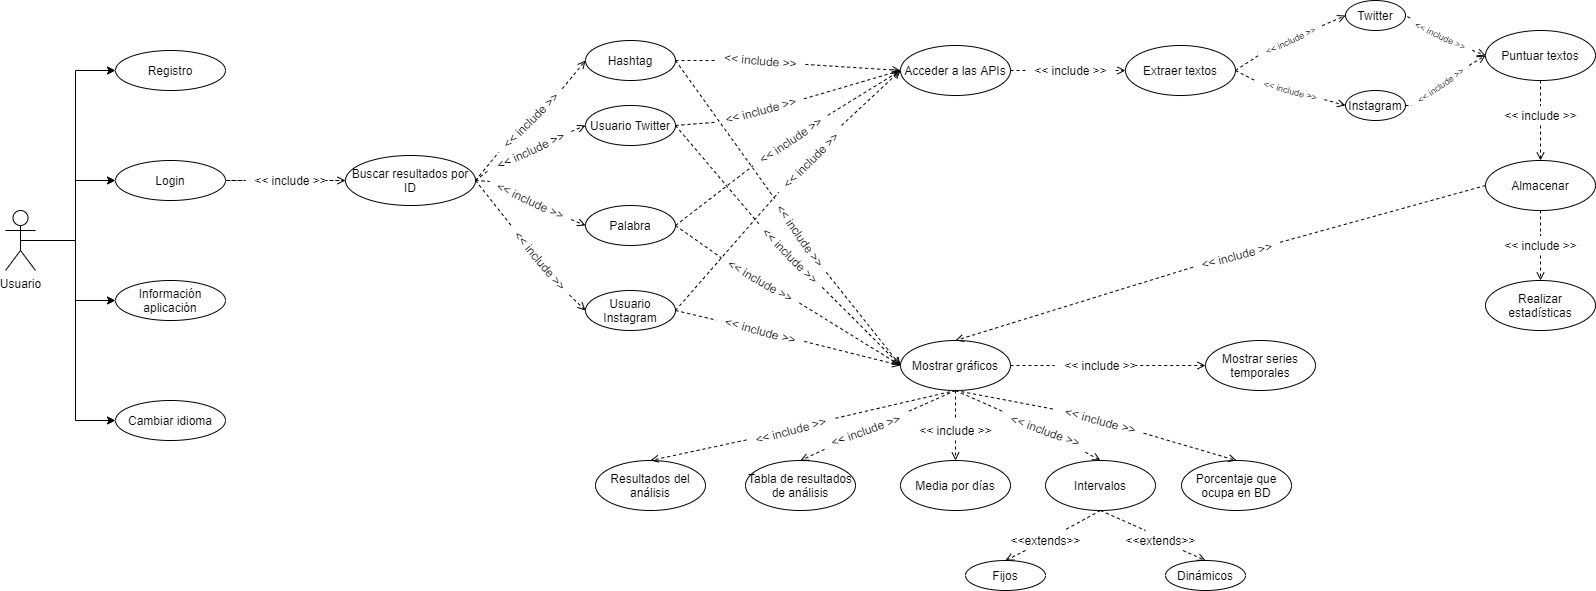
\includegraphics[scale=0.45]{img/CUSentinel.jpg}
    \caption{Diagrama de casos de uso}
\end{figure}
\end{landscape}





\apendice{Especificación de diseño}

\section{Introducción}
En este apartado se explica cómo se han organizado y diseñado las diferentes partes de la aplicación.

\section{Diseño de datos}
La base de datos de la aplicación cuenta con diferentes tablas:

\begin{itemize}\tightlist
    \item \textbf{Register:} En esta tabla se almacenan todos los usuarios registrados. Para crear una cuenta el usuario debe introducir su nombre, apellido, nombre que quiere dar a la cuenta y la contraseña. La tabla además tiene un identificador que es un autoincremental.
    \item \textbf{Datahashtags:} Almacena los hashtags con la fecha de creación, los tweets donde aparece y el valor del análisis. 
    \item \textbf{Datausertw:} Guarda los resultados de los tweets referentes a un usuario, el tweet en el que ha sido nombrado, la fecha del tweet y el valor del análisis.
    \item \textbf{Dataword:} En ella se almacenan las palabras buscadas junto con los tweets en los que aparece esa palabra, la fecha en la que se escribieron y el análisis de los tweets.
    \item \textbf{Datauserig:} Guarda todos los comentarios que se han realizado en el perfil del usuario buscado junto con la fecha de estos y el resultado del análisis.
    \item \textbf{Statistics:} En esta tabla se almacenan cada hashtag, usuario de twitter, palabra o usuario de instagram junto con la media, moda, mediana, varianza y desviación típica del conjunto de sus resultados.
\end{itemize}

\imagen{Esquema_BD}{Esquema de la base de datos.}

\newpage
\section{Diseño procedimental}
En este apartado se muestra la ejecución de la aplicación mediante varios diagramas de secuencia.

\subsection{Registro y Login}
El primer diagrama de secuencia representa los pasos que sigue el programa en el momento en el que el usuario se registra y después accede a la aplicación con su cuenta.

\imagen{img/sequence_diagram/sequence_diagram_login_register.png}{Diagrama de secuencia de Registro y Login}

\newpage
\subsection{Análisis en twitter}
En este diagrama podemos ver la ejecución del programa cuando se realiza el análisis en la opción de twitter.

\imagen{img/sequence_diagram/sequence_diagram_tw.jpg}{Diagrama de secuencia de Análisis en twitter}

\newpage
\subsection{Análisis en instagram}
Aquí podemos observar los pasos al ejecutar una orden de análisis en instagram. 

\imagen{img/sequence_diagram/sequence_diagram_ig.jpg}{Diagrama de secuencia de Análisis en instagram}

\newpage
\section{Diseño arquitectónico}
En este apartado se explicarán los diferentes patrones de diseño que se han utilizado para que la aplicación tenga un buen diseño software y esto ayude a la mantenibilidad de esta.

\subsection{Modelo-Vista-Controlador (MVC)}
En este patrón como su nombre indica las partes del \textbf{modelo}, los datos de la aplicación, la \textbf{vista}, representación de los datos y el \textbf{controlador}, encargado de reaccionar a las entradas del usuario, están bien diferenciadas y relacionadas entre ellas. \cite{apuntesMVC}

En nuestra aplicación cada componente abarca:
\begin{itemize}\tightlist
    \item \textbf{Modelo:} Está compuesto por los módulos de instagram, twitter, statistics\_formulas y database. En estos módulos se realizan todas las operaciones para extraer los datos de las APIs, se calcula el sentimiento de los resultados y se almacena todo en la base de datos.
    \item \textbf{Vista:} Es la interfaz de usuario, es la parte con la que el usuario interactúa y le muestra toda la información. Se ha realizado en angular y se trata de varios componentes que realizan comunicaciones con el controlador para poder comunicarse entre distintas ventanas, mostrar gráficos, etc.
    \item\textbf{Controlador:} Es el módulo denominado server. Se encarga de todas las comunicaciones con los servicios de la vista. Este recoge las peticiones que se hacen desde la interfaz y llama a los diferentes módulos para realizar las operaciones y devolver un json con la información deseada.
\end{itemize}

\imagen{patrones/mvc}{Patrón MVC. \cite{ImgMVC}}

\subsection{Fachada}
Este patrón tiene como función dar una interfaz unificada de alto nivel al cliente, aunque por debajo este formado por varias interfaces. \cite{patronFachada}

En nuestro caso el patrón fachada se utiliza para 'ocultar' a la interfaz de usuario los módulos que realmente hacen las operaciones, es decir, los módulos de twitter, instagram, database y statistics\_formulas. En ellos se realizan todas las operaciones y se comunican entre ellos para poder almacenar los resultados en la base de datos. Sin embargo, la interfaz de usuario no conoce de su existencia, ya que solamente se comunica con el módulo server que en este caso hace la función de fachada. El módulo server es el que conoce toda la estructura, porque se comunica con ambas partes, ya que los módulos que realizan las operaciones tampoco tienen conocimiento de la existencia de la fachada, pues no tienen ninguna dependencia hacia ella. 

\imagen{patrones/fachada}{Patrón Fachada.}

\clearpage
\section{Diseño de interfaces}
Al principio del proyecto, en la semana tres se realizó un prototipo de la interfaz de la aplicación. Para ello se utilizó la herramienta Pencil.

\imagen{prototipo_interfaz}{Prototipo de interfaz.}

Este prototipo nos sirvió para hacernos una idea de como enfocar la aplicación a nivel de usuario, aunque se han modificado algunas cosas para la interfaz final, la estructura es casi la misma.

Cuando se empezó con la parte visual de la aplicación se decidió que era mejor buscar una plantilla y modificarla a nuestro gusto, para que las ventanas de la aplicación se unificaran.

\newpage
Se ha utilizado una plantilla para la estructura de ventanas como login, menú, la portada, etc. Para la ventana de gráficos se buscó en la misma web una plantilla específica para este componente que se asemejara a la plantilla del resto de la aplicación. El resultado final es el siguiente:

\imagen{interfazreal}{Interfaz final.}




\apendice{Documentación técnica de programación}

\section{Introducción}
En este apéndice se va a explicar cómo está organizado el proyecto, el manual del programador y los requisitos necesarios para poder ejecutar el proyecto. 

\section{Estructura de directorios}
En el proyecto hay cuatro directorios principales:
\begin{itemize}
\tightlist
    \item\textbf{frontend:} Es el directorio donde se encuentra todo el código de Angular con el que se ha realizado la interfaz de la aplicación y las conexiones con el código de python.
    \item\textbf{src:} Aquí se alojan todos los archivos python, que son los que realizan la gestión de la aplicación.
    \item\textbf{ux\_ui:} En esta carpeta se aloja el prototipo que se realizó al principio del proyecto de cómo iba a ser la aplicación.
    \item\textbf{doc:} En este directorio encontramos los documentos de la memoria y los anexos, junto con sus imágenes y complementos.
\end{itemize}
\newpage
\subsection{frontend}
Dentro de este directorio como hemos indicado anteriormente se encuentran todo el código que crea la interfaz y la conecta con el código de python.
Dentro de ella podemos encontrar dos subdirectorios:
\begin{itemize}
\tightlist
    \item\textbf{e2e:} Contiene configuración de angular.
    \item\textbf{src:} Contiene el código en typescript, los archivos css y las imágenes.
\end{itemize}

\subsubsection{frontend/src}
Contiene tres subdirectorios:
\begin{itemize}
\tightlist
    \item src/app: Contiene todos los componentes que generan la interfaz. Hay un componente por cada página de la aplicación.
    \item src/assets: Aloja todos los archivos css y las imágenes utilizadas en la aplicación.
\end{itemize}


\section{Manual del programador}

\subsection{Instalación de Python}
Para ejecutar nuestro proyecto es necesario instalar Python, para ello podemos descargar la versión aquí: \url{https://www.python.org/downloads/}
Cuando la descarga haya finalizado ejecutamos e instalamos.

\subsection{Instalación de MySQL}
En MySQL es necesario descargar MySQL Workbench y MySQL Server. Para ello iremos a la página oficial, \url{https://dev.mysql.com/downloads/} y descargaremos el MySQL Installer.
Cuando lo ejecutamos, hay que seguir las instrucciones y añadir los complementos. También hay que instalar el MySQL Connector Python.

\subsection{Instalación de Nodejs}
Para la parte de angular es necesario instalar Nodejs, por tanto accederemos a la página oficial, \url{https://nodejs.org/es/download/}, y descargaremos la versión que necesitemos y llevaremos a cabo su instalación.

Tras la instalación de los distintos elementos es recomendable reiniciar el equipo para que no haya problemas de compatibilidad, ya que por ejemplo, MySQL Connector Python necesita que tengamos instalado Python, y puede darse que si no reiniciamos el equipo no lo detecte.

\section{Compilación, instalación y ejecución del proyecto}
Para la utilización del proyecto, se debe descargar del repositorio de GitHub en el que está subido \url{https://github.com/ZoeCalvo/Sentinel}, lo descomprimimos y ya podemos comenzar.
El proyecto ha sido realizado con la herramienta de PyCharm, su instalación es opcional ya que se puede ejecutar desde la consola de comandos.

En caso de que instalemos PyCharm:

\subsection{Importar y ejecutar en PyCharm}
Debemos abrir la herramienta y seleccionar \textit{File>Open} escogemos el proyecto y aceptamos.
Tardar unos minutos en generar los esquemas e importar todo. 
Cuando ya hayamos realizado esto, deberemos instalar varias librerías de Python que se irán marcando en rojo.
Si usamos PyCharm, posicionando el ratón encima de la librería nos sugerirá instalar el paquete, seleccionamos que sí y comenzará la instalación.

Las librerías que necesitan instalación son:

\subsection{Librerías de Python}
Las primeras librerías necesarias serán \textit{Flask y Flask\-Cors}, ya que la aplicación utiliza el framework Flask.
Cors se utiliza para que las conexiones entre páginas no causen problema.

Para poder acceder a Instagram, nos hemos instalado una librería de un repositorio de GitHub.
Para Twitter hay que instalar la librería \textit{tweepy.py}

En cuanto al análisis de sentimientos, se ha utilizado un repositorio de GitHub \url{https://github.com/aylliote/senti-py.git}, lo descomprimimos y para instalarlo debemos instalar \textit{spanish\_sentiment\_analysis}.

Para los análisis en inglés, tenemos la librería TextBlob que es la que hemos utilizado para el análisis y Yandex Translate, que lo hemos utilizado para la detección del idioma.

Para el cálculo de series temporales se han utilizado las librerías \textit{statsmodels y pmdarima}, cuya instalación también es necesaria.

Para realizar la instalación de cada una de las librerías, en consola se realizará con el comando \textit{pip install} seguido de la librería.


\subsection{Instalación de Angular}
Tras realizar la instalación de Nodejs, para poder construir el proyecto de angular debemos ejecutar una serie de comandos.

Primero, en una consola nos posicionamos en la ruta del proyecto de angular, en nuestro caso sería dentro de la carpeta \textit{frontend}.
Ejecutamos el comando \textit{npm install -g @angular/cli} que va a instalar las dependencias de angular/cli.
Tardará unos minutos, cuando termine ejecutaremos \textit{npm install} lo que va a instalar todos los módulos de node que tenemos indicados en el archivo \textit{package.json}.
Para finalizar levantaremos el proyecto con \textit{npm start}, este comando compila el proyecto y lo levanta en \url{http://localhost:4200/}.

Esto es necesario solo para la primera vez que se instala el proyecto.

\subsection{Ejecución del proyecto}
Cuando el proyecto ya se ha levantado una vez, para poder correr la aplicación deberemos abrir dos consolas, en las cuales accederemos dentro del proyecto de esta forma:

$$\textit{cd \{path\}}$$

En la primera consola, estando ya dentro de la ruta del proyecto escribiremos lo siguiente:

$$\textit{cd src}$$
$$\textit{py server.py}$$

Con ello ejecutaremos el servidor.

En la segunda consola escribiremos:

$$\textit{cd frontend}$$
$$\textit{ng serve}$$

Esto iniciará nuestro proyecto en \url{http://localhost:4200/}

Mientras estemos utilizando la aplicación no debemos cerrar ninguna de las dos consolas ya que esto parará su ejecución.

La aplicación necesita algunas credenciales, las cuales se han introducido en variables de entorno para que no sean públicas en el repositorio, por tanto si no están declaradas en variables de entorno, la aplicación no se ejecutará.

\subsection{Máquina Virtual}
Si se utiliza la máquina virtual que se proporciona, el PIN de acceso es: \textit{1a2b}.

\apendice{Documentación de usuario}

\section{Introducción}
En este apéndice se va a explicar cómo ejecutar la aplicación por parte del usuario.

\section{Requisitos de usuarios}
La aplicación va a ser accesible desde este enlace \url{https://frontsentinel.herokuapp.com/}. 
La aplicación ha sido desplegada y está operativa para el hosting gratuito, pero para poder disponer de ella de forma más rápida, ya que conlleva gran carga de almacenamiento, se facilita una máquina virtual con todos los requisitos ya instalados. De esta forma, se podrán realizar pruebas más rápidas.

Como se trata de una aplicación web, no es necesario que el usuario cuente con más requisitos que tener una versión del navegador compatible:

\begin{itemize}
\tightlist
    \item Safari 9 o superior.
    \item Opera 28 o superior.
    \item Google Chrome 41 o superior.
    \item Mozilla Firefox 40 o superior.
    \item Microsoft Edge 12 o superior.
\end{itemize}



\section{Instalación}
El usuario no va necesitar instalar nada para poder utilizar Sentinel, simplemente debe utilizar un navegador de los anteriores y acceder al enlace.

\section{Manual del usuario}
Para el manual de usuario se ha realizado una wiki en español e inglés, está accesible a través de este enlace: 
\url{https://zcs0001.gitbook.io/sentinel/}

Como se ha explicado en los requisitos, para acceder a la aplicación se puede hacer a través del enlace \url{https://frontsentinel.herokuapp.com/}, o a través de la máquina virtual facilitada.

\subsection{Inicio}
Esta es la primera página que se visualiza cuando se entra en la web, en ella aparece el nombre de la aplicación, de qué trata en una frase y el nombre de la autora.

\imagen{/manual_usuario/inicioES}{Página de inicio de la aplicación.}

\subsection{Barra de navegación}
Este elemento está presente en todas las ventanas de la aplicación y es el que va a permitir al usuario comenzar a interactuar con la web.
Contiene tres botones y un menú desplegable. 
El primer botón es \textbf{SENTINEL} que al pulsarlo nos redirigirá a la pantalla de inicio.
El botón \textbf{INFORMACIÓN} nos lleva a la página en la que se explica de forma general la aplicación y cómo utilizarla.
El botón \textbf{LOGIN}, es el que nos dará acceso a la pantalla en la que podremos introducir nuestro usuario y contraseña para acceder al menú de la aplicación.
Además, cuenta con un menú desplegable para poder cambiar de idioma. Como se puede ver, la aplicación está disponible en inglés y en castellano.
 
\imagen{/manual_usuario/navbarES}{Barra de navegación.}

\subsection{Información}
En la ventana de información se encuentra una breve explicación de qué es Sentinel y cuáles son sus objetivos.

Cuenta con una lista de cuales son los cinco pasos que te permitirán utilizar de forma correcta la web y se cuenta de donde nace la idea de la herramienta.

Además dentro de la página se adjuntan fotos de como es la aplicación, pantalla de inicio y gráficos.

\imagen{/manual_usuario/info1ES}{Página de información primera parte.}
\imagen{/manual_usuario/info2ES}{Página de información segunda parte.}

\subsection{Login}
En caso de ser la primera vez que se utiliza la web, hay un botón de \textbf{CREAR CUENTA} que nos redirigirá a la ventana del registro.

Para poder acceder al menú hay que introducir el nombre de usuario y contraseña.

En caso de que la cuenta exista, nos mostrará una notificación emergente de bienvenida. En caso contrario mostrará una diciendo que el usuario o la contraseña no son correctos.

\imagen{/manual_usuario/loginES}{Página de login.}

\imagen{/manual_usuario/accesoES}{Acceso permitido.}

\imagen{/manual_usuario/noaccesoES}{Acceso denegado.}

\subsection{Registro}
Tras haber seleccionado el botón de \textbf{CREAR CUENTA} en la ventana de Login aparece la ventana en la que podremos registrarnos.
Para realizar el registro hay que rellenar los campos que nos aparecen que son: nuestro nombre, apellido, el nombre de usuario que queramos utilizar y la contraseña.
Después de rellenar el formulario pulsamos el botón de \textbf{REGISTRARSE} y si no hemos introducido ningún carácter inválido nos redirigirá a la ventana de \textbf{LOGIN} de nuevo para que realicemos el acceso.

\imagen{/manual_usuario/registroES}{Página de registro.}

Para los campos de nombre y apellidos solo se permiten letras mayúsculas y minúsculas. Para el nombre de usuario y la contraseña además de letras mayúsculas y minúsculas se pueden añadir números enteros y guiones bajos.

En caso de introducir un carácter no permitido se mostrará una alerta.

\imagen{/manual_usuario/letramalregistroES}{Carácter no permitido.}

\subsection{Menú}
Cuando realizamos el acceso correctamente la web nos redirige a la ventana del menú, donde podemos elegir en qué red social queremos analizar.
Tenemos la opción de analizar en Twitter o en Instagram, para acceder a cualquiera de las dos, podemos seleccionar el botón o la imagen, ya que ambas dan acceso a la ventana de análisis.

\imagen{/manual_usuario/menuES}{Página de menú.}

\subsection{Ventana de análisis en Twitter e Instagram}
La ventana de análisis en Twitter y la de análisis en Instagram son iguales excepto en los caracteres que se permiten en el identificador, por ello se han juntado.
Podemos ver que tienen un formulario en el cual nos piden el identificador por el que queremos buscar y las fechas entre las que queremos buscar. Además una casilla en la que podemos solicitar que se actualicen los resultados de la base de datos.
Para realizar el análisis lo único que es indispensable es el identificador, la fecha es opcional ya que si no introducimos ninguna se nos mostrarán todos los resultados que hay en la base de datos de ese identificador.

\imagen{/manual_usuario/instagramES}{Página de análisis en instagram.}

\imagen{/manual_usuario/twitterES}{Página de análisis en twitter.}

En el análisis de Twitter el identificador que puede introducirse es un hashtag, un usuario o una palabra.
\begin{itemize}
\tightlist
    \item \textbf{Hashtag:} Para buscar un hashtag hay que introducir el símbolo \# antes de la palabra. Por ejemplo \textit{\#ubu}. 
    \imagen{/manual_usuario/hashtag}{Hashtag.}
    \item \textbf{Usuario:} Si queremos buscar sobre un usuario hay que escribir lo primero @ seguido del nombre del usuario. Por ejemplo \textit{@UBUEstudiantes}.
    \imagen{/manual_usuario/userTw}{Usuario de twitter.}
    \item\textbf{Palabra:} En este caso simplemente se debe introducir la palabra. 
    \imagen{/manual_usuario/palabra}{Palabra.}
\end{itemize}
En el análisis de Instagram solo se puede buscar sobre un usuario, por lo que en el identificador deberemos introducir el usuario pero sin @.

\imagen{/manual_usuario/userIg}{Usuario de instagram.}

Si escribimos algún carácter que no sea permitido, nos mostrará un mensaje de error.

\imagen{/manual_usuario/errorTWES}{Carácter incorrecto para twitter.}
\imagen{/manual_usuario/errorIGES}{Carácter incorrecto para instagram.}

Para seleccionar fechas hay que seleccionar la casilla y se desplegará un calendario para que escojamos una fecha.

\imagen{/manual_usuario/selectDate}{Escoger una fecha.}

Cuando hayamos introducido todo se nos redirigirá a la ventana de gráficos para mostrar los resultados.

\subsubsection{Actualizar base de datos}
Cuando vamos a realizar el análisis la aplicación nos permite actualizar los resultados que están almacenados en la base de datos para poder tener datos más actuales.
Si queremos seleccionar esta opción, deberemos marcar la casilla de Actualizar base de datos.
Entonces, nos aparecerá una alerta de que la acción podría tardar unos minutos. Cuando termine de cargar los nuevos resultados nos redirigirá automáticamente a la ventana de gráficos.

\imagen{/manual_usuario/updateBDES}{Actualizar la base de datos.}

\subsubsection{El identificador no está en la base de datos}
Cuando buscamos un identificador que no se encuentra en la base de datos previamente la aplicación mostrará una alerta de que la acción puede tardar unos minutos. Por tanto, hay que esperar y cuando se hayan cargado los resultados se nos redirigirá a la ventana de gráficos de forma automática.

\imagen{/manual_usuario/noIDES}{El identificador no está en la base de datos.}

\subsection{Gráficos}
En esta pantalla se muestran los resultados de la búsqueda en gráficos para poder tener una experiencia más visual.
Además de los gráficos, nos permite el acceso a la pantalla de series temporales. Este botón se encuentra en la parte superior a la derecha. También hay un botón para poder volver al menú y así realizar un análisis nuevo que se encuentra en la parte inferior a la izquierda.

\imagen{/manual_usuario/accesoTSES}{Botón para acceder a series temporales.}

\imagen{/manual_usuario/volvermenuES}{Botón para volver al menú.}

Hay varios gráficos y tablas, a continuación se explica cada uno

\subsubsection{Resultados de análisis-Gráfico}
Es un gráfico de barras que nos muestra todos los resultados del análisis, su fecha y su puntuación.

\imagen{/manual_usuario/resultsAnalisisES}{Gráfico de los resultados del análisis.}

\subsubsection{Media por días}
Este gráfico de líneas nos muestra el resultado de realizar la media por días.

\imagen{/manual_usuario/mediaxdiaES}{Gráfico de la media por día.}

\subsubsection{Gráfico de intervalos}
Es un gráfico de barras que agrupa los resultados en intervalos de 0.1. Los intervalos son fijos entre el -1 y el 1.

\imagen{/manual_usuario/intervalosfijosES}{Gráfico de intervalos fijos.}

Si seleccionamos el icono de intervalos dinámicos que aparece debajo del gráfico, se nos mostrarán los resultados agrupados en intervalos calculados de forma dinámica. Es decir, serán diez intervalos entre el menor valor de los resultados y el mayor.

\imagen{/manual_usuario/intervalosdinamicosES}{Gráfico de intervalos dinámicos.}

\subsubsection{Sentinel Trends}

Es un gráfico circular que nos muestra la importancia que tiene el identificador en nuestra base de datos, ya que se calcula cuántos resultados hay respecto al total.

\imagen{/manual_usuario/sentinelTrendsES}{Gráfico de sentinel trends.}

\subsubsection{Resultados de análisis-Tabla}
Esta tabla nos muestra los resultados del análisis y el texto que se ha analizado.

\imagen{/manual_usuario/analisisTabla}{Tabla de los resultados del análisis.}

\subsubsection{Estadísticas}
En esta tabla se nos muestra el identificador que hemos buscado junto con los cálculos estadísticos que se han realizado a los resultados. Las operaciones estadísticas realizadas son media, mediana, moda, varianza y desviación típica.

\imagen{/manual_usuario/tablaestadisticasES}{Tabla de estadísticas.}

\subsection{Series Temporales}
En esta ventana podemos calcular series temporales a partir de los resultados recogidos del identificador. 
Se muestra un menú en el que hay que elegir qué serie temporal queremos, el modelo y una casilla en la que pondremos cuántos valores queremos predecir.

\imagen{/manual_usuario/menuTSES}{Menú de series temporales.}

También tenemos un botón en la parte inferior a la izquierda para volver al menú.

\imagen{/manual_usuario/volvermenuES}{Botón para volver al menú.}

\subsubsection{Desplegable serie temporal}
Nos dan tres opciones de series temporales a calcular, suavizado exponencial, método Holt y método Arima.

\imagen{/manual_usuario/tsTipoES}{Desplegable serie temporal.}

\subsubsection{Desplegable modelo}
Se puede elegir entre el modelo aditivo o multiplicativo.

\imagen{/manual_usuario/modeloES}{Desplegable modelo.}

\subsubsection{Valores a predecir}
Tenemos una casilla para introducir un valor entero positivo de cuántos valores queremos predecir. Además cuenta con flechas para aumentar el valor por si no queremos escribir el valor.

\imagen{/manual_usuario/prediccionES}{Valores a predecir.}

Cuando hayamos seleccionado una opción en cada uno pulsaremos el botón de calcular, lo cual nos mostrará los resultados.

Lo primero, nos muestra si la serie temporal es o no estacionaria.

\imagen{/manual_usuario/estacionariaES}{Es o no estacionaria.}

Después se nos muestran cuatro gráficos.

\subsubsection{Serie temporal}
Este gráfico nos muestra los resultados reales, en la línea verde, los resultados de calcular la serie temporal en naranja y los valores de predicción en azul.

\imagen{/manual_usuario/TSgraficoES}{Gráfico de serie temporal.}

Los tres gráficos restantes resultan de descomponer la serie temporal.

\subsubsection{Estacionalidad}
En este gráfico se muestra la estacionalidad de la serie temporal, es decir, su variación a lo largo del tiempo.

\imagen{/manual_usuario/estacionalidadES}{Gráfico de la estacionalidad.}

\subsubsection{Tendencia}
La gráfica muestra la tendencia de la serie temporal que refleja la evolución a largo plazo.

\imagen{/manual_usuario/TendenciaES}{Gráfico de la tendencia.}

\subsubsection{Residuo}
En este gráfico vemos el residuo de la serie temporal, que se usa para probar el grado de ajuste de los modelos.

\imagen{/manual_usuario/residuoES}{Gráfico del residuo.}





\bibliographystyle{plain}
\bibliography{bibliografiaAnexos}

\end{document}
